\documentclass[12pt]{beamer}
\mode<presentation>
\usepackage{setup}
\usepackage{subfigure}
\usepackage[lined]{algorithm2e}
\usepackage[small]{caption}
\usepackage[utf8x]{inputenc}
\usepackage{default}
\usepackage{tikz}
\usepackage{cite}
\usepackage{amsfonts}
\usepackage{amssymb}
\usepackage{graphicx}
\usepackage{subcaption}
\usepackage{algorithm2e}
\usepackage{microtype}
\usepackage{color, colortbl}
\usepackage{subcaption}
\usepackage{url}
\usepackage{multirow}
\usepackage{amsmath,amsthm, amsfonts,amssymb}


%\nobibliography{refs}
\title{Approximate Clustering Algorithms for High Dimensional Streaming and Distributed Data}
\author{A Dissertation Defense by: \\
Lee A. Carraher}
\institute[UMBC]{
  Department of Electrical Engineering and Computing Systems\\
  University of Cincinnati \\
}
\date{\today}

\begin{document}
\addtobeamertemplate{navigation symbols}{}{%
    \usebeamerfont{footline}%
    \usebeamercolor[fg]{footline}%
    \hspace{1em}
    \insertframenumber/\inserttotalframenumber
}

%----------- titlepage ----------------------------------------------%
\begin{frame}[plain]
  \titlepage
\end{frame}

\begin{frame}[plain]{Agenda}
\begin{itemize}
 \item Classification Problem
 \item Data Analysis and Clustering
 \item Research Goals Motivation and Hypothesis
 \item Related Work and Background
 \item RPHash and Streaming RPHash Algorithms
 \item Experimental Setup, First comparisons
 \item Adaptive LSH and Tree-Walk Improvement
 \item Experiments with TWRP
 \item Conclusions and Future Directions
\end{itemize}
\end{frame}

\begin{frame}[plain]{Problem Introduction}
\begin{itemize}
  \item Animals evolved to classify
  \item classification tasks for survival
  \begin{itemize}
      \item edible, predator, suitable mate
  \end{itemize}
  \item Can't experience everything
  \item Instead need models based on attributes
  \begin{itemize}
      \item teeth size?, leaf shape?, is an engineer?
  \end{itemize}
  \item Humans are good classifiers for some things 
\end{itemize}
\end{frame}

\begin{frame}[plain]{Classifiers}
    \begin{figure}
        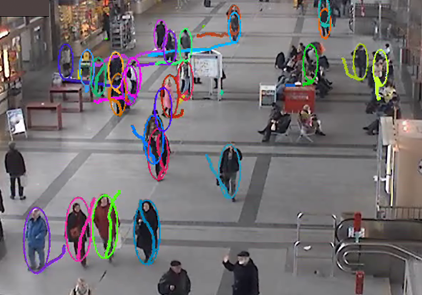
\includegraphics[width=.8\textwidth]{figs/people.png}
    \end{figure}
    We are good at identifying people.
  \end{frame}

\begin{frame}[plain]{Classifiers}  
    \begin{figure}
        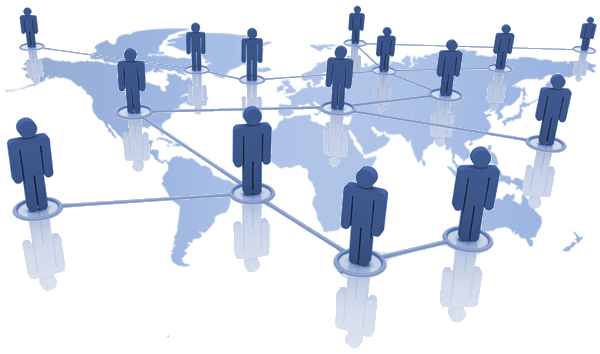
\includegraphics[width=.8\textwidth]{figs/social.png}
    \end{figure}
    Not good at large global networking tasks.
\end{frame}

\begin{frame}[plain]{Classifiers}  
    \begin{figure}
        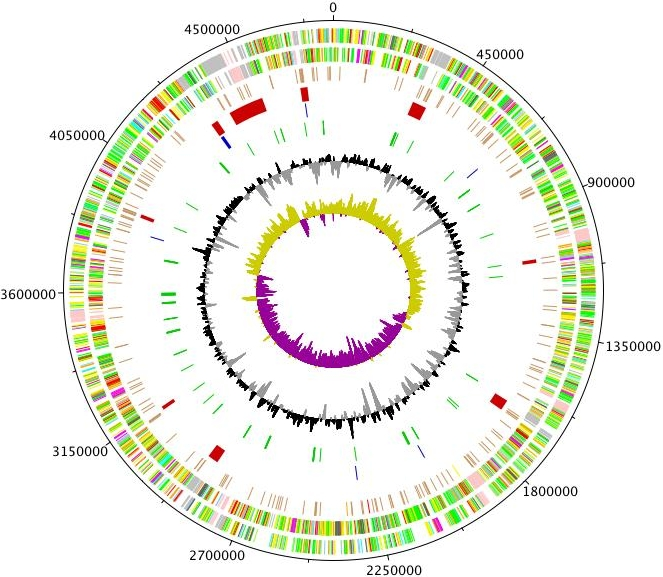
\includegraphics[width=.6\textwidth]{figs/Styphi.jpg}
    \end{figure}
    Or abstract data clustering tasks.
\end{frame}

\begin{frame}[plain]{Classifiers}
    
\begin{itemize}
 \item We are good at classify things we experience
 \item Not good at classifying numerical data
 \item Not good at classifying large data
 \begin{itemize}
  \item  $\#$ groups,  $\#$ attributes
 \end{itemize}
\item Not good at classifying unfamiliar things (EKG, Subatomic Interactions...)
\end{itemize}
\end{frame}

\begin{frame}[plain]{Example Problem}

 A researcher wants to track the geographic dependence or independence, of a particular medical condition.
 However the patient data reside in disconnected, separately managed databases. The data contains a wide variety
 of symptoms and biometric measures, for millions of patients. There is an additional constrain placed on the data 
 due to its private and personally identifying nature. 
 \begin{itemize}
  \item grouping the symptoms and referencing location could prove or disprove this claim
  \item high dimensional data
  \item geographically separated data
  \item private individually identifiable data
 \end{itemize}
\end{frame}

\begin{frame}[plain]{Data Analysis}
  \begin{itemize}
    \item Data Analysis can provide insights into data that often go beyond human cognition
  \begin{itemize}
    \item Data with complex relationships (financial trans.)
    \item Things foreign to us (subatomic, galactic objects)
    \item Lots of fast moving things (tweets)
  \end{itemize}
    \item How do we create models for these things?
  \end{itemize}
\end{frame}


\begin{frame}[plain]{Data Clustering}
\begin{itemize}
 \item Data clustering builds models for classification
 \item Cluster Models capture similarities between observation attributes
 \item Clustering is a classic Machine Learning Problem
 \item The $k$-Means Problem is a clustering problem
\end{itemize}
\end{frame}

\begin{frame}[plain]{$k$-means Problem}
\centering
\textbf{$4$-means}
\begin{figure}
 \centerline{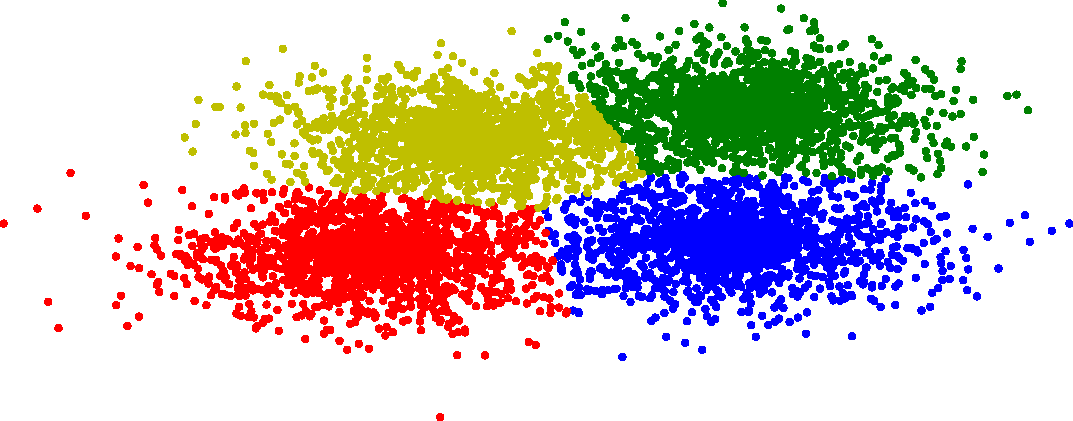
\includegraphics[width=.7\textwidth]{figs/kmean}}
\end{figure}
\vspace*{-3\bigskipamount}
 \begin{itemize}
  \item partition observations into $k$ subsets
  \item group observations with similar attributes
  \item an optimization problem: maximize some objective either inter-cluster or intra-cluster
 \end{itemize}
\end{frame}


\begin{frame}[plain]{$k$-Means Conti.}
\begin{Theorem}[Clustering Objective Function]
 $$
{\underset{C}{\text{argmin}}} {\overset{k}{\sum}} {\underset{x\in C}{\sum}} ||x-\mu_i||^2
$$
\end{Theorem}
\begin{itemize}
 \item \textbf{$k$-Means} $\in$\textbf{Max-SNP}$\in$\textbf{APX}$\in$\textbf{NP},
 \item \textbf{APX} are approximable by \textbf{PTAS}
\end{itemize}
\end{frame}

\begin{frame}[plain]{Growth of Big Data}

 Data sets are growing fast
 \begin{itemize}
  \item Medical, Scientific, Financial, Social, Security
 \end{itemize}
  \begin{figure}
 \centerline{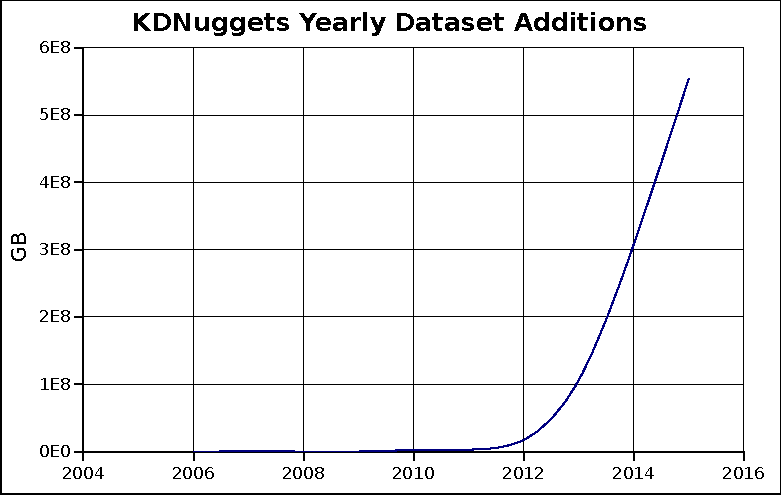
\includegraphics[width=.7\textwidth]{figs/datasetsizes}}
\end{figure}
\vspace*{-3\bigskipamount}
\begin{itemize}
 \item Some are $\infty$(unbounded) $\rightarrow$  streaming data model.
\end{itemize}
\end{frame}

\begin{frame}[plain]{What needs to be solved?}
  \begin{itemize}
   \item PTAS is good complexity for small problems
   \item Big Data problems require lower complexity
   \item Streaming algorithms put addition requirements on space
   \item If we distribute data, are the connections trustworthy? 
   \begin{itemize}
    \item Need security
   \end{itemize}
  \end{itemize}
\end{frame}



\begin{frame}[plain]{Goals}
\begin{itemize}
\item A distributable $k$-means clustering algorithm.
\item A streaming $k$-means clustering algorithm.
\item Compare clustering performance to other algorithms.
\item Show a sub-quadratic complexity growth.
\item Evaluate dataset security.
\item Experiment with approximate components of RPHash
\end{itemize}
* same as the proposal
\end{frame}

\begin{frame}[plain]{Motivation of RPHash}
RPHash is a degenerate case of Locality Sensitive Hash (LSH) based $cr$-NN
\begin{itemize}
  \item $cr$-NN: given a query x return the k nearest neighbors
\end{itemize}
\begin{Definition}[Nearest Neighbor] \cite{Samet}\\
Given a set of vectors $P$ in $R^d$ and query vector $q$ return $k$ vectors $p\subseteq P$ such that
$p=\text{Argmin}\{dist(p',q)\}$, where dist is some metric function.
\end{Definition}
\end{frame}

\begin{frame}[plain]{LSH NN}

\begin{columns}
      \begin{column}{.5\linewidth}
	Build the DB:\\
	\vspace*{1\bigskipamount}
	\RestyleAlgo{boxruled}
	%\caption{Preprocessing on Dataset X \label{lshnn}}
	\DontPrintSemicolon
	\ForAll{$x \in X$} 
	{	id = LSH\_Hash(x)\\
		$T$[id].add$(x)$\\
	}
	\textbf{Return:} $T$
      \end{column}
      
      \begin{column}{.5\linewidth}
	  Query the DB:\\
	  \vspace*{1.5\bigskipamount}
	  \RestyleAlgo{boxruled}
	  %\caption{Query $k$ nearest to $q$ in X, using hashtable $T$\label{lshnnq}}
	  \DontPrintSemicolon
	  id = LSH\_Hash($q$)\\
	  \textbf{Return:} linear\_scan($T$[id],$k$)\\
      \end{column}
\end{columns}

\end{frame}


\begin{frame}[plain]{LSH NN}
\begin{itemize}
  \item LSH NN: LSH to narrow search
  \item Works well in practice!
  \item Not so well if LSH buckets contain many points
  \item But can be viewed as centroid candidates
\end{itemize}
\end{frame}


\begin{frame}[plain]{Hypothesis}
\begin{itemize}
  \item Degenerate LSH is useful for Clustering
  \item Combine Random Projection with LSH gives us an approximate dense region sampling
  \item Approximate Clustering is equivalent to local minima clustering
  %\item Storing a sketch of data gives similar results to storing entire data
  %\item The resulting set of algorithms are called: \\\emph{Random Projection Hash} (\emph{RPHash}).
  %\begin{itemize}
  %  \item \emph{RPHash} is comparable to similar $k$-Means algorithms in performance
  %  \item \emph{RPHash} is scalable and distributable
  %  \item \emph{RPHash} can maintain security of distributed data
  %\end{itemize}
  \end{itemize}
\end{frame}

\begin{frame}[plain]{Related Work}
\begin{itemize}
 \item Standard algorithm classes
 \begin{itemize}
  \item $k$-means(Lloyd), mean-shift, agglomerative, spectral
 \end{itemize}
 \item tend to have bad scalability complexity
 \item Focus on $k$-means(Lloyd) type
 \end{itemize}
 \begin{itemize}
  \item Tree Based Clustering\cite{Liu2000}
 \end{itemize}

 \end{frame}
 
 \begin{frame}[plain]{Scalable Clustering Related Work}
  \begin{itemize}
    \item Projection based clustering
    \begin{itemize}
      \item Proclus - project to lower dim.
      \item Cluster Ensemble - Histograms
    \end{itemize}
    \item Density scanning clustering algorithms
    \begin{itemize}
    \item DBScan
    \item Clique
    \item CLARANS
    \end{itemize}
  \end{itemize}
\end{frame}
 
\begin{frame}[plain]{Stream Clustering Related Work}
    \begin{itemize}
      \item CSketch - most similar
      \item Streaming $k$-Means - similar structure
      \item Damped Sliding Window
      \item DStream
      \item Biased Reservoir Sampling
    \end{itemize}
\end{frame}

\begin{frame}[plain]{Algorithm Outline}
In this thesis we present 3 algorithms for large scale distributed data clustering, that
stem from the same basic setup.
 \begin{itemize}
  \item Random Projection Hash (RPHash)
  \item Streaming RPHash
  \item Tree-Walk RPHash (TWRP)
 \end{itemize}
\end{frame}

\begin{frame}[plain]{\emph{RPHash} Components}
\begin{itemize}
   \item Random Projection 
   \item Locality Sensitive Hashing
   \item Exact and approximate counting
   \item Off-line clustering
  \end{itemize}
\end{frame}

\begin{frame}[plain]{Random Projection}
\begin{itemize}
 \item Use Random Projection to mitigate Curse of Dimensionality and enforce data embeddings

\item JL-Lemma
$d \approx \mathlarger{\mathlarger{\mathlarger{\Omega}}} \left( \frac{log(m)}{\epsilon^2 log(1/\epsilon)} \right)   $
  \item $d$ can be even lower for clustering tasks (Bartal '11)
  \item bonus, unrecoverable data anonymization (Liu,Kargupta,Ryan '06)%\footnote{\bibentry{rppriv}}
  \item Gaussian RP, DB friendly, and FJLT Projection
\end{itemize}
\end{frame}

\begin{frame}[plain]{LSH Function}

 \begin{Definition}[Locality Sensitive Hash Function]
let $\mathbb{H}=\{h:S \rightarrow U\}$ is $(r_1,r_2,p_1,p_2)-$sensitive if for 
any $u,v\in S$
 \begin{enumerate}
   \item if $d(u,v) \leq r_1$ then $Pr_{\mathbb{H}}[h(u)=h(v)]\geq p_1$
   \item if $d(u,v) > r_2$ then $Pr_{\mathbb{H}}[h(u)=h(v)]\leq p_2$
 \end{enumerate}
\end{Definition}
\begin{itemize}
 \item We increase selectivity by appending LSH function results
 \item And decrease prob. of missing NN by probing many times
\end{itemize}

\end{frame}

\begin{frame}[plain]{Real World LSH}
Lattice Based LSH
\begin{itemize}
 \item Leech Lattice ($\Lambda_{24}$) - optimal regular lattice partitioning in $\mathbb{R}^{24}$
 \item $E_8$ - optimal regular lattice partitioning in $\mathbb{R}^{8}$
 \item $D_n$ - checkerboard lattice
\end{itemize}
Other LSH
\begin{itemize}
 \item Spherical - force data to lie on the partitioned surface of a hypersphere
 \item P-stable - partition orthogonal projections of a vector with a stable distribution
 \item $k$-means - use the dual of $k$-means centroids to define the space partitioning
\end{itemize}
\end{frame}


\begin{frame}[plain]{LSH Based Clustering}
 \begin{figure}
 \centerline{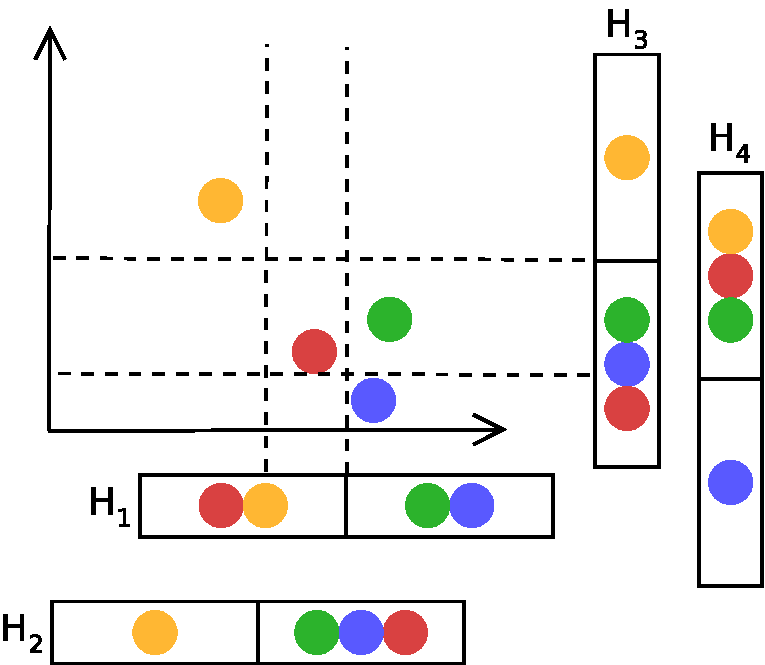
\includegraphics[width=.7\textwidth]{figs/multiLSHClustering}}
\end{figure}
\end{frame}


\begin{frame}[plain]{Data Prerequisites}
\begin{itemize}
    \item  $k$ - number of clusters\\
    \item$X=\{x_1, \dots, x_n\}$, $x_k \in \mathbb{R}^m$ - set of data vectors\\
    \item  $\mathbb{H}(\cdot)$ - LSH Function with bucket radius=$r$, dim=$d$\\
    \item  $\mathbb{P} = \{p_1,...p_n\}$ - set of $n, m \times d $ matrices w/ \emph{JL} property\\
    \item$C:h \rightarrow 0$ - empty map of hashes to counts\\
    \item$M : h\rightarrow \langle0, \dots, 0\rangle$ - empty map of hashes to vectors\\
    \item clusterer($M,k$) - a standard clustering algorithm
  \end{itemize}
\end{frame}

\begin{frame}[plain]{Phase 1: Counting Dense Regions}
  %\begin{algorithm}
  %  \caption{\emph{RPHash} Algorithm Phase 1\label{\emph{RPHash}Phase1}}
    \ForAll{$x_k \in X$} 
    {
      \ForAll{$p_i \in \mathbb{P}$} 
      {
	$\tilde{x_k}\leftarrow  \sqrt{\frac{m}{d}}p_i^{\intercal}x_k $\\ %\tcp*{projection}
	$t = \mathbb{H}(\tilde{x_k})$\\%\tcp*{LSH}
	$C[h]+=1$\\%\tcp*{increment count} 
      }
    }
    $C$.sort()\\%\tcp*{descending sort by count}
    \KwResult{$C[0:k*P.length]$)}%\tcp*{truncate the map}}
  %\end{algorithm}
\end{frame}

\begin{frame}[plain]{Phase 2: Cluster Assignment}

%\begin{algorithm}
%\caption{\emph{RPHash} Algorithm Phase 2\label{\emph{RPHash}Phase2}}
\ForAll{$x_k \in X$}
{
  \ForAll{$p_i \in \mathbb{P}$} 
  {
    $\tilde{x_k}\leftarrow \sqrt{\frac{m}{d}}p_i^{\intercal}x_k $\\%\tcp*{projection}
    $h =  \mathbb{H}(\tilde{x_k})$\\%\tcp*{blur and LSH}
    \If{$h \cap C$.keys $ = \emptyset$}
    {
	$\Delta = M[h]-x_k$%\tcp*{weighted vec.}
	$M[h]=M[h]+\Delta/C[h]$  %\tcp*{update}
    }
  }
}
 \KwResult{clusterer($M,k$) \tcp*{merge centroids}}
%\end{algorithm}
\end{frame}

\begin{frame}[plain]{Streaming Model}
\begin{figure}
 \centerline{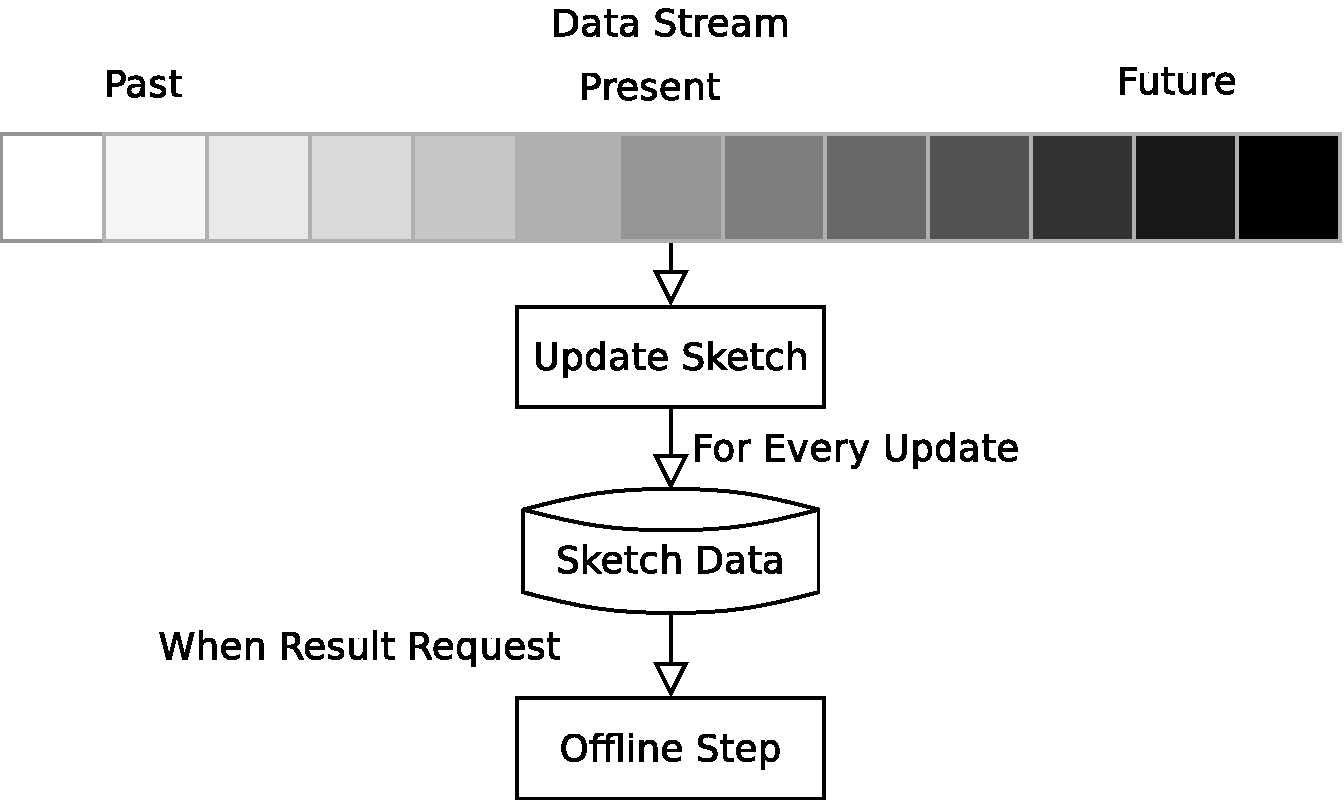
\includegraphics[width=.65\textwidth]{figs/Streaming}}
\end{figure}
\vspace*{2\bigskipamount}
\begin{itemize}
 \item Data arrives as a stream
 \item No random access to all data vectors 
 \item data stream is unbounded
 \begin{itemize}
 \item algorithm must be sub-quadratic
 \end{itemize}
 \item Strict Memory bound
\end{itemize}
\end{frame}

\begin{frame}[plain]{CountMin Sketch Structure}
    \begin{center}
      \begin{figure}
	\centerline{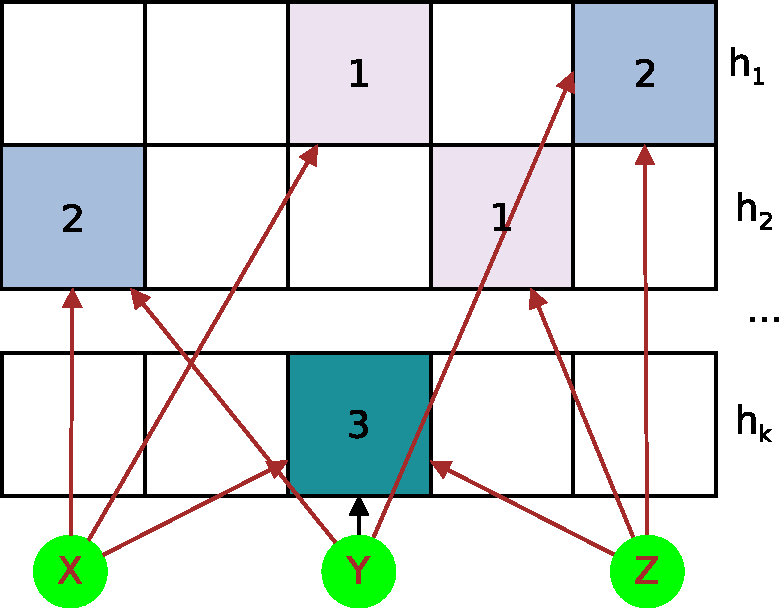
\includegraphics[width=.65\textwidth]{figs/countmin}}
      \end{figure}
    \end{center}
    \end{frame}

\begin{frame}[plain]{Streaming RPHash Diagram}
 \begin{figure}
 \centerline{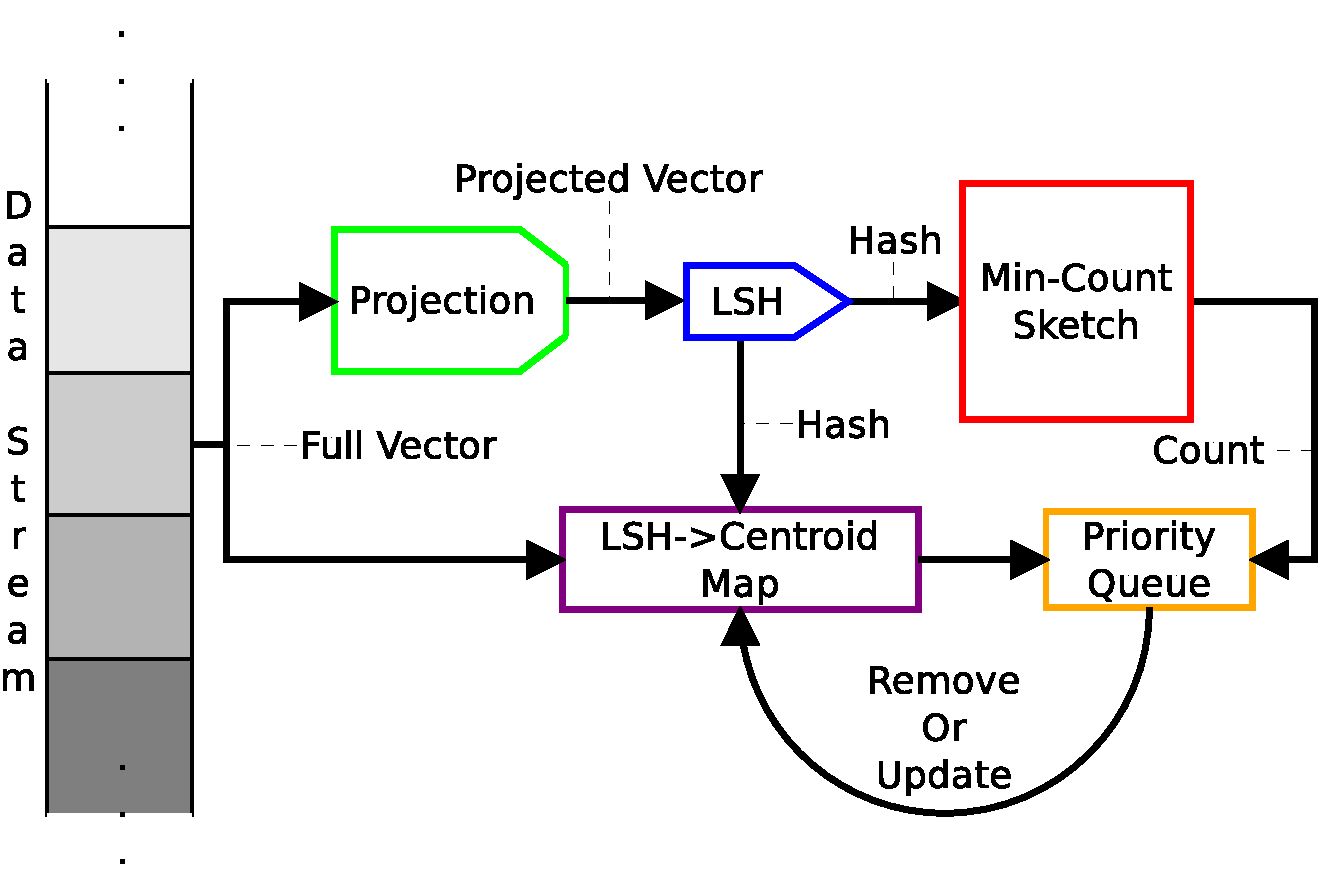
\includegraphics[width=.7\textwidth]{figs/rphashoverview}}
\end{figure}
\end{frame}

\begin{frame}[plain]{Streaming Algorithm}
  \textbf{Data} \\
\begin{itemize}
    \item  $k$ - number of clusters\\
    \item  $x \in\mathbb{R}^m$ - data vector from stream\\
    \item  $\mathbb{H}(\cdot)$ - LSH Function radius=$r$, dim=$d$\\
    \item  $\mathbb{P} = m \times d $ matrix w/ \emph{JL} property\\
    \item  $M$- lsh\_key $\rightarrow$ centroid map \\
    \item  $C$- cm-sketch data structure \\
    \item  $T$- CM-Sketch based $\epsilon k$ bounded priority queue\\
\end{itemize}
\end{frame}

\begin{frame}[plain]{Add Next Vector}
  \ForAll{$x \in X$} 
  {
    $\tilde{x}:= \sqrt{\frac{m}{d}}p^{\intercal}x$ \\%\tcp*{Random Projection}
    $t := \mathbb{H}(\tilde{x})$ %\tcp*{LSH Hashing}
    $C$.add$(t)$\\
    \eIf{$t\in M$.keys}
    {
      $M[t].wadd(x)$  %\tcp*{Weighted add}
    }
    {
	$M[t]=$new centroid($x$,C.count(t))\\
	$T$.insert$(M[t])$\\
    }
    M.remove(T.pop())  %\tcp*{remove least}
  }
\end{frame}

\begin{frame}[plain]{First Round Experiments}
 \begin{itemize}
 \item Define evaluation metrics
 \item Review Datasets
 \begin{itemize}
  \item Real World
  \item Synthetic
 \end{itemize}
 \item Optimize RPHash Configuration Parameters
 \item Algorithms for Comparison
 \item Standard RPHash Results
 \item Streaming Results
\end{itemize}
\end{frame}

\begin{frame}[plain]{Experiment Metrics}
 \begin{itemize}
  \item Internal performance metrics - unlabeled metrics
  \begin{itemize}
    \item WCSSE - within cluster sum of squares
  \end{itemize}
  \item External performance metrics - require ground truth labels
  \begin{itemize}
    \item ARI - Adjusted Rand Index
    \item Cluster Purity
  \end{itemize}
  \item Runtime
  \item Memory Consumption
 \end{itemize}
\end{frame}

\begin{frame}[plain]{Datasets}
\begin{itemize}
 \item Synthetic data generators in R and Java
 \begin{itemize}
   \item Uniformly Distributed Models
   \item Uneven sized clusters
   \item Gaussian distributed vectors
   \item Sparse
   \item Noise injected
\end{itemize}
\end{itemize}
\vspace*{-2\bigskipamount}
 \begin{table}
\centering
\resizebox{\columnwidth}{!}{
\begin{tabular}{|l|r|r|r|l|}
\hline
\rowcolor[HTML]{FFCE93} 
\textbf{Data Set} & \textbf{Num of}   & \textbf{Num of}   & \textbf{Num of} & \textbf{Type of} \\
\rowcolor[HTML]{FFCE93}
                  & \textbf{Clusters} & \textbf{Features} & \textbf{Vectors} & \textbf{Data} \\ \hline
Arrhythmia \cite{guvenir-xx}     & 16 &  279 &   452 & Real   \\
CNAE-9 \cite{ciarelli-xx}        &  9 &  856 &  1080 & Binary \\
Cora \cite{sen-08}               &  7 & 1433 &  2708 & Binary \\
Gisette \cite{guyon-04}          &  2 & 5000 &  7000 & Real   \\
Human Activity \cite{anguita-13} &  6 &  561 & 10299 & Real   \\
UJIIndoorLoc \cite{sospedra-14}  &  3 &  520 & 21000 & Real   \\
WebKB \cite{sen-08}              &  5 & 1703 &   265 & Binary \\ \hline
\end{tabular}
}
\end{table}
\end{frame}

\begin{frame}[plain]{RPHash Parameter Study}
\centering
6400 Configurations!
 \begin{table}
\centering
\resizebox{\columnwidth}{!}{
\begin{tabular}{|c|c|c|c|c|}
\hline
\rowcolor[HTML]{D1FF99} 
\textbf{\emph{LSH} Algorithm} & \textbf{Projected Dimension(s)} & \textbf{\# Projections} & \textbf{\# Blurrings} & \textbf{Offline Clustering} \\ \hline
$E_8$                         & 8              & & & \\ \cline{1-2}
Multi-$E_8$                   & 8, 16, 24, 32  & & & \\ \cline{1-2}
Leech                         & 24             & & & \\ \cline{1-2}
Multi-Leech                   & 24, 48, 72, 96 & & & \\ \cline{1-2}
\emph{L\'{e}vy} $p$-stable    &                & & & \\ \cline{1-1}
\emph{Cauchy} $p$-stable      &                & & & \\ \cline{1-1}
\emph{Gaussian} $p$-stable    &                & & & \\ \cline{1-1}
Spherical                     & \multirow{-4}{*}{8, 16, 24, ..., 80} & \multirow{-8}{*}{1, 2, 3, ..., 8}  & \multirow{-8}{*}{1, 2, 3, 4} & \multirow{-8}{*}{\begin{tabular}[c]{@{}c@{}}$k$-means\\Single Linkage\\ Complete Linkage\\ Average Linkage\end{tabular}} \\ \hline
\end{tabular}
}
\end{table}
\end{frame}

\begin{frame}[plain]{Best Configurations}
\begin{figure}
 \centerline{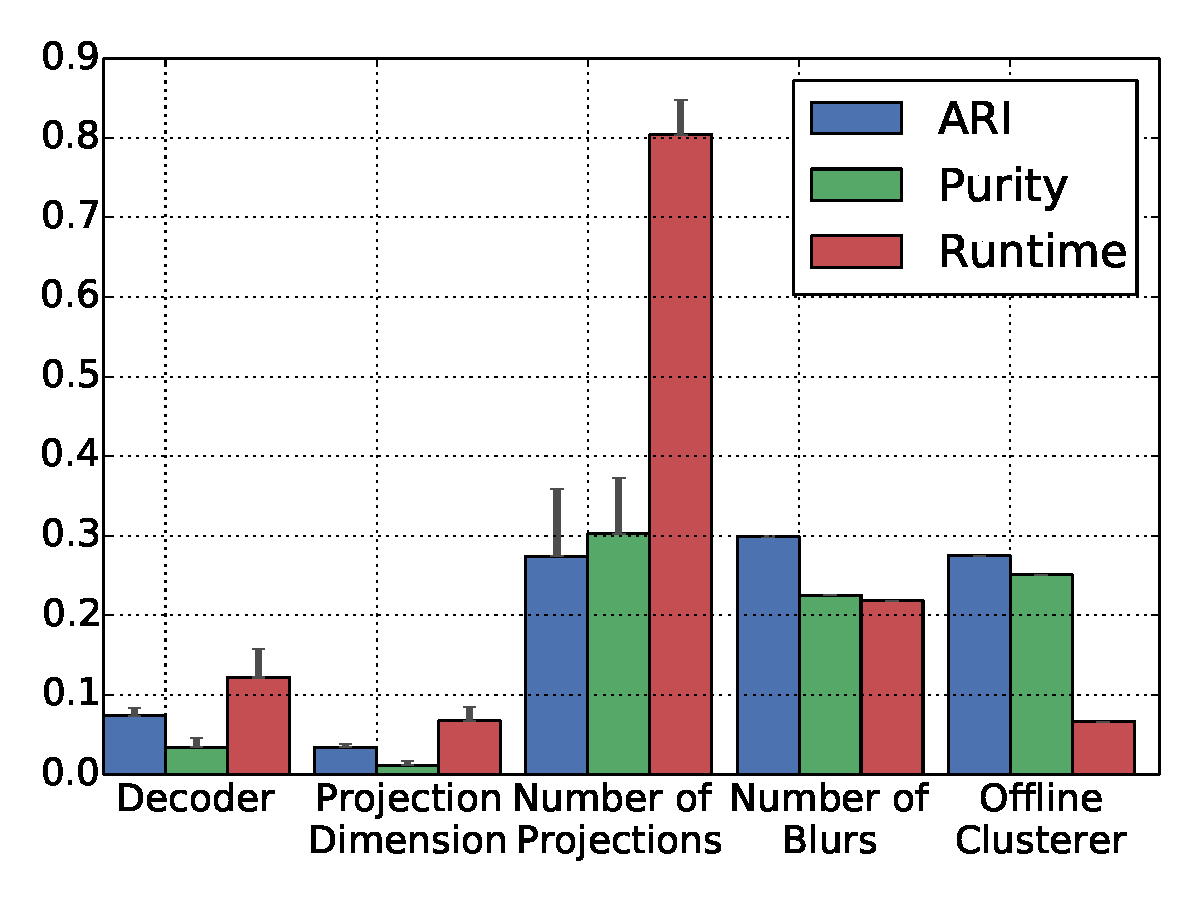
\includegraphics[width=.5\textwidth]{figs/correlation}}
\end{figure}
\vspace*{-3\bigskipamount}
 \begin{table}
\centering
\resizebox{\columnwidth}{!}{%
\begin{tabular}{|l|l|c|c|c|c|c|c|c|c|}
\hline
\rowcolor[HTML]{FFFFC7} 
\textbf{Data Set} & \textbf{Configuration} & \multicolumn{4}{|c|}{\textbf{\textsf{RPHash}}} & \multicolumn{4}{|c|}{\textbf{$k$-means}} \\
\rowcolor[HTML]{FFFFC7} 
 & & \textbf{ARI} & \textbf{Purity} & \textbf{Runtime} & \textbf{Memory} & \multicolumn{1}{|c}{\textbf{ARI}} & \textbf{Purity} & \textbf{Runtime} & \textbf{Memory} \\  \hline
Arrhythmia
& Multi-$E_8$/24/1/2/Complete Linkage  & 0.2710 & 0.5885 & 0.1277 & 0.1420 & 0.0811 & 0.6069 & 0.5287 & 16.4333 \\
CNAE-9
 & Multi-Leech/72/5/2/$k$-means        & 0.3424 & 0.5707 & 0.7917 & 0.8312 & 0.2798 & 0.5312 & 2.7120 & 165.1167 \\
Cora
 & Multi-Leech/96/3/3/Complete Linkage & 0.1065 & 0.3988 & 2.6022 & 0.6660 & 0.1158 & 0.4271 & 52.410 & 227.9833 \\
Gisette
& Spherical/16/2/3/$k$-means           & 0.5675 & 0.6218 & 1.7769 & 0.4530 & 0.4610 & 0.6002 & 24.746 & 1485.0667 \\
UJIIndoorLoc
 & Spherical/8/8/2/$k$-means           & 0.6608 & 0.8268 & 1.3840 & 0.2780 & 0.6954 & 0.7750 & 23.821 & 2850.6500 \\
WebKB
 & Spherical/16/5/1/$k$-means          & 0.4210 & 0.7396 & 0.1117 & 0.9015 & 0.4403 & 0.7528 & 0.8087 &   50.1500 \\ \hline
\end{tabular}
}
\end{table}
\end{frame}

\begin{frame}[plain]{Comparison algorithms}
Static Clustering:
\begin{itemize}
 \item \textbf{$k$-Means:} \cite{Hartigan}.\label{clusteralgos} 
 \item \textbf{Agglomerative Hierarchical clustering:} Single, Complete, Average and Ward's method. 
\item \textbf{Self-organizing Tree Algorithm (SOTA):} \cite{Herrero}.
\item \textbf{$k$-Means++} \cite{arthur-07}
\end{itemize}
Streaming Clustering
\label{streamingalgos}
\begin{itemize}
 \item \textbf{Streaming $k$-Means:} \cite{braverman}
 \item \textbf{Damped Sliding Window:} \cite{zhu}
 \item \textbf{DStream:} \cite{dstream}
 \item \textbf{Biased Reservoir Sampling:} \cite{ccaggarwal}
\end{itemize}
\end{frame}

\begin{frame}[plain]{Experiments: Real Data}
 \begin{figure}
\begin{table}
\centering
\resizebox{\columnwidth}{!}{%
\begin{tabular}{|c|c|c|c|c|c|c|c|c|}
\hline
\rowcolor[HTML]{FFFFC7} 
\textbf{Data Set} & \textbf{Measures} & \cellcolor[HTML]{D1FF99}\textbf{\textsf{RPHash}} &
  \textbf{$k$-means} \cite{Hartigan} & \textbf{Single} & \textbf{Complete} & \textbf{Average} &
  \textbf{Ward's} & \textbf{SOTA} \cite{Herrero} \\ 
\rowcolor[HTML]{FFFFC7}
& & & & \textbf{Linkage} & \textbf{Linkage} & \textbf{Linkage} & \textbf{Method} \cite{Murtagh} &  \\ \hline
 & ARI     & 0.0697 &     0.0811 &    0.0461 &    0.0963 &    0.0546 &    0.0889 &    0.0981 \\
 & Purity  & 0.6058 &     0.6069 &    0.5730 &    0.5885 &    0.5752 &    0.5951 &    0.6062 \\
 & Runtime & 0.2709 &     0.5287 &    0.1680 &    0.1640 &    0.1680 &    0.1680 &    3.4440 \\
\multirow{-4}{*}{Arrhythmia}
 & Memory  & 0.7070 &    16.4333 &    3.4000 &    3.4000 &    3.4000 &    3.4000 &   21.3000 \\ \hline
 & ARI     & 0.2788 &     0.2798 &    0.0000 &    0.0000 &    0.0000 &    0.3547 &    0.1730 \\
 & Purity  & 0.4873 &     0.5312 &    0.1185 &    0.1204 &    0.1185 &    0.5722 &    0.3657 \\
 & Runtime & 0.3932 &     2.7120 &    4.3360 &    4.3400 &    4.3400 &    4.3440 &    3.7080 \\
\multirow{-4}{*}{CNAE-9}
 & Memory  & 1.1370 &   165.1167 &   24.2000 &   24.2000 &   24.2000 &   24.1000 &  134.2000 \\ \hline
 & ARI     & 0.0915 &     0.1158 &    0.0001 &    0.0120 &    0.0002 &    0.0930 &    0.0647 \\
 & Purity  & 0.3858 &     0.4271 &    0.3039 &    0.3335 &    0.3039 &    0.4597 &    0.3342 \\
 & Runtime & 0.8290 &    52.4100 &   71.9200 &   71.9600 &   71.9400 &   71.9720 &   11.7120 \\
\multirow{-4}{*}{Cora}
 & Memory  & 1.4590 &   227.9833 &  100.7000 &  100.7000 &  100.7000 &  100.7000 &  265.4000 \\ \hline
 & ARI     & 0.1282 &     0.0615 &    0.0000 &    0.0000 &    0.0000 &    0.0018 &    0.1147 \\
 & Purity  & 0.6720 &     0.6241 &    0.5001 &    0.5003 &    0.5001 &    0.5216 &    0.6694 \\
 & Runtime & 2.7363 &   423.7660 & 2280.4320 & 2280.4640 & 2280.0800 & 2280.5480 &   46.8120 \\
\multirow{-4}{*}{Gisette}
 & Memory  & 1.4300 &  2138.3833 &  829.3000 &  829.3000 &  829.3000 &  829.3000 & 2097.5000 \\ \hline
 & ARI     & 0.3348 &     0.4610 &    0.0000 &    0.3270 &    0.3321 &    0.4909 &    0.3143 \\
 & Purity  & 0.4631 &     0.6002 &    0.1890 &    0.3770 &    0.3588 &    0.6597 &    0.3966 \\
 & Runtime & 1.8774 &    24.7460 &  413.8800 &  414.3320 &  414.0960 &  414.4480 &   14.2440 \\
\multirow{-4}{*}{HAR}
 & Memory  & 0.5157 &  1485.0667 & 1259.0000 & 1214.9000 & 1214.8000 & 1214.9000 &  946.2000 \\ \hline
 & ARI     & 0.5043 &     0.6954 &    0.0001 &    0.0001 &    0.0001 &    0.6021 &    0.3351 \\
 & Purity  & 0.7105 &     0.7750 &    0.4635 &    0.4635 &    0.4635 &    0.7732 &    0.6918 \\
 & Runtime & 2.6363 &    23.8213 & 1093.9440 & 1094.7000 & 1094.8200 & 1095.5360 &   16.1880 \\
\multirow{-4}{*}{UJIIndoorLoc}
  & Memory  & 0.2460 & 2850.6500 & 5132.4000 & 5049.0000 & 5049.0000 & 5049.0000 & 2227.0000 \\ \hline
  & ARI     & 0.3205 &    0.4403 &    0.0066 &    0.0404 &    0.0066 &    0.3276 &    0.3906 \\
  & Purity  & 0.7063 &    0.7528 &    0.4755 &    0.5283 &    0.4755 &    0.7094 &    0.7019 \\
  & Runtime & 0.1648 &    0.8087 &    0.3760 &    0.3760 &    0.3760 &    0.3760 &    2.5400 \\
\multirow{-4}{*}{WebKB}
 & Memory  & 1.2000 &    50.1500 &    6.3000 &    6.4000 &    6.3000 &    6.3000 &   44.1000 \\ \hline
\end{tabular}
}
\end{table}
\end{figure}
\end{frame}

\begin{frame}[plain]{Streaming RPHash}
 \begin{itemize}
  \item Test on UJII Indoor Localization
  \item High Dimensional (d=561)
  \item Many observation (21000)
 \end{itemize}
\end{frame}


\begin{frame}[plain]{Streaming RPHash}
\begin{figure}
 \centerline{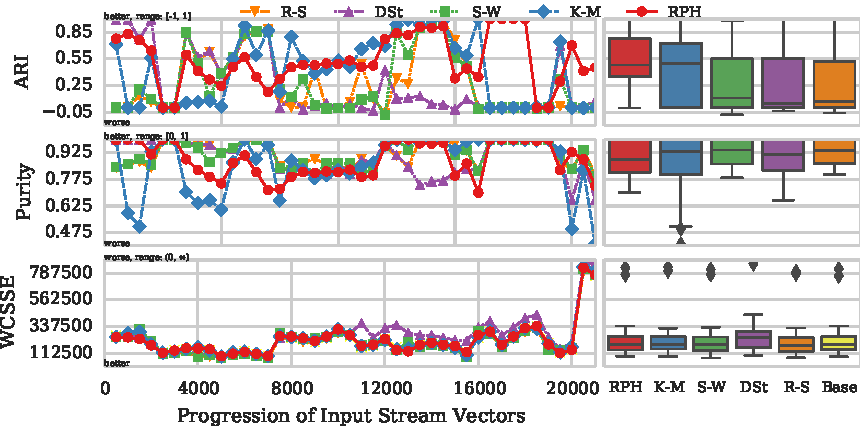
\includegraphics[width=1.\textwidth]{figs/resultsUJII}}
\end{figure}
\end{frame}

\begin{frame}[plain]{Streaming RPHash}
\begin{figure}
 \centerline{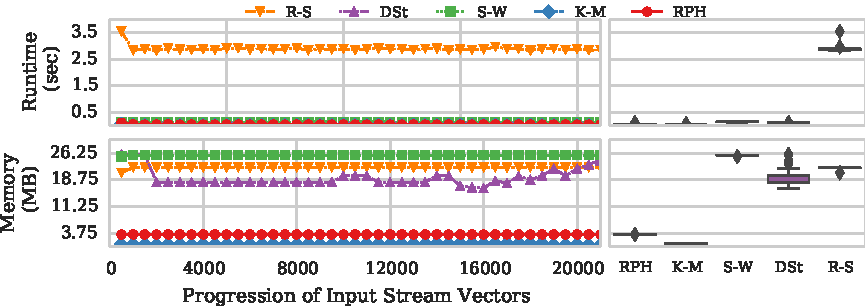
\includegraphics[width=1.\textwidth]{figs/runtimeUJII}}
\end{figure}
\end{frame}

\begin{frame}[plain]{Streaming RPHash}
\begin{figure}
 \centerline{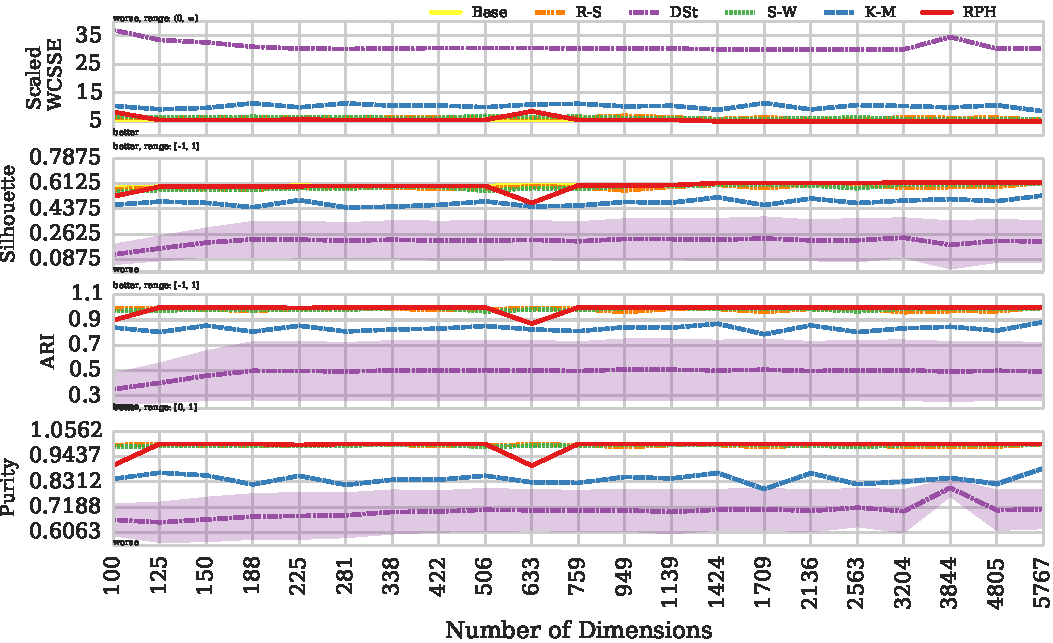
\includegraphics[width=1.\textwidth]{figs/measure_scale}}
\end{figure}
\end{frame}

\begin{frame}[plain]{Performance Instability}
\begin{figure}
 \centerline{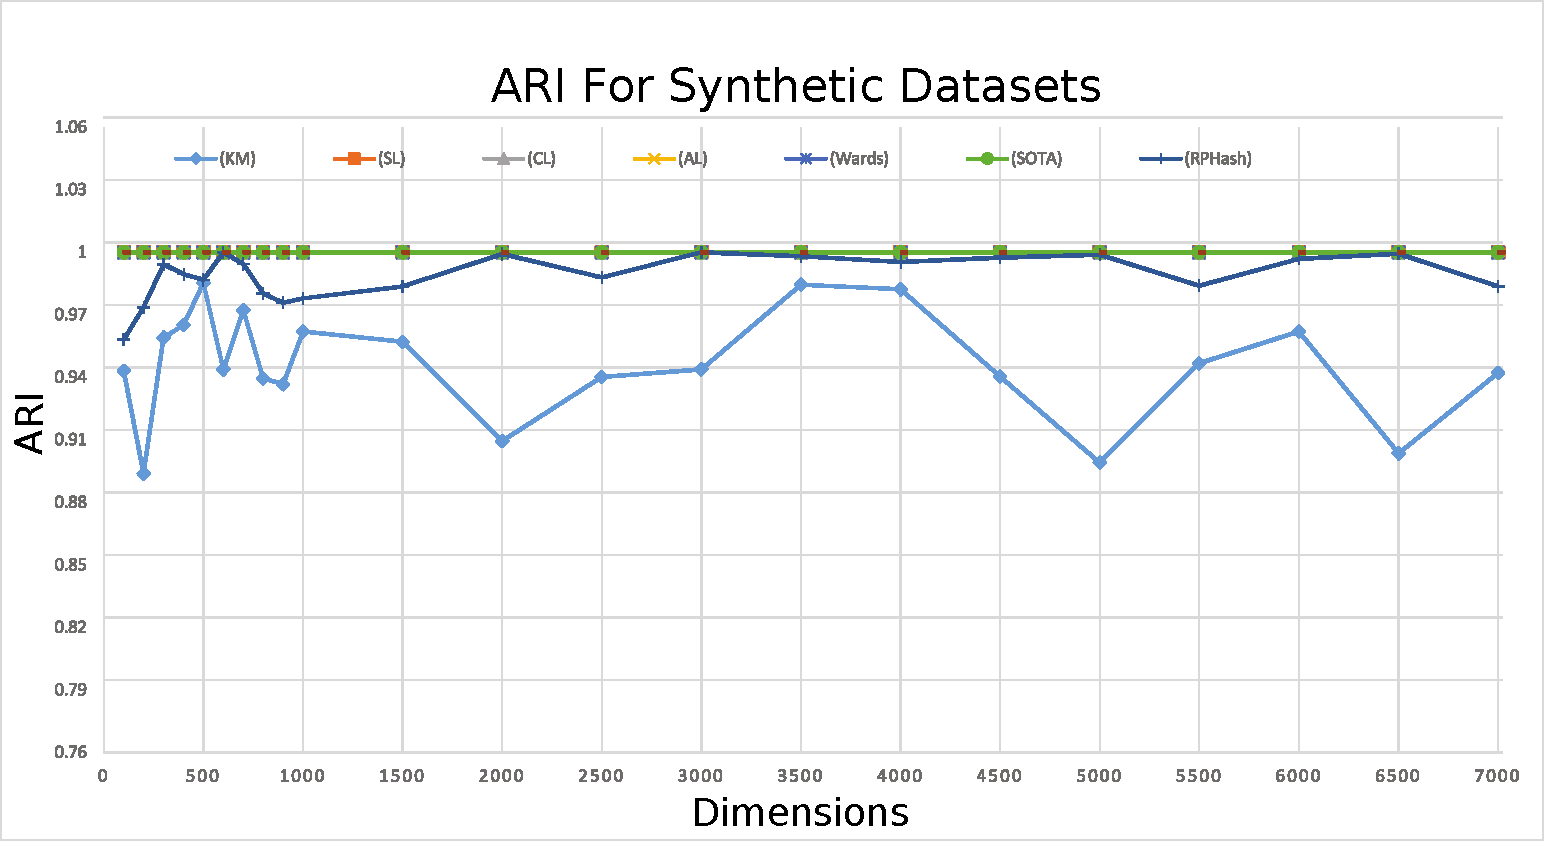
\includegraphics[width=1.\textwidth]{figs/ari_synthetic}}
\end{figure}
\vspace*{-3\bigskipamount}
\begin{itemize}
 \item RPHash and $k$-Means Results are unstable
 \item Testing shows that RP and Counting are not the problem
 \item Problem must lie in the LSH Function
\end{itemize}
\end{frame}

\begin{frame}[plain]{Better LSH}
Fix The LSH Functions
 \begin{itemize}
  \item LSH functions are good when data is uniformly distributed
  \item clusterable data by definition is not uniformly distributed
  \item use a set of nested hash functions to adapt to data
 \end{itemize}
 \begin{Definition}[LSH Composability]
 An LSH function $\mathbb{H}^n(x)$ that maps $x \in \mathbb{R}^n \rightarrow \mathbb{Z}^n_2$,
 is composable if there is a related function $\mathbb{H}^{n-1}(x_{n-1})$ that maps $x_{n-1} \in \mathbb{R}^{n-1} \rightarrow \mathbb{Z}^{n-1}_2$
 where
 $\mathbb{H}^{n-1}(x_{n-1}) = \big(\mathbb{H}^n(x)+1\big) \bigcup \big(\mathbb{H}^n(x)+0\big) $ 
 for all $x_{n} \in \mathbb{R}^{n}$
\end{Definition}
\end{frame}

\begin{frame}[plain]{Adaptive LSH}
\begin{figure}
 \centerline{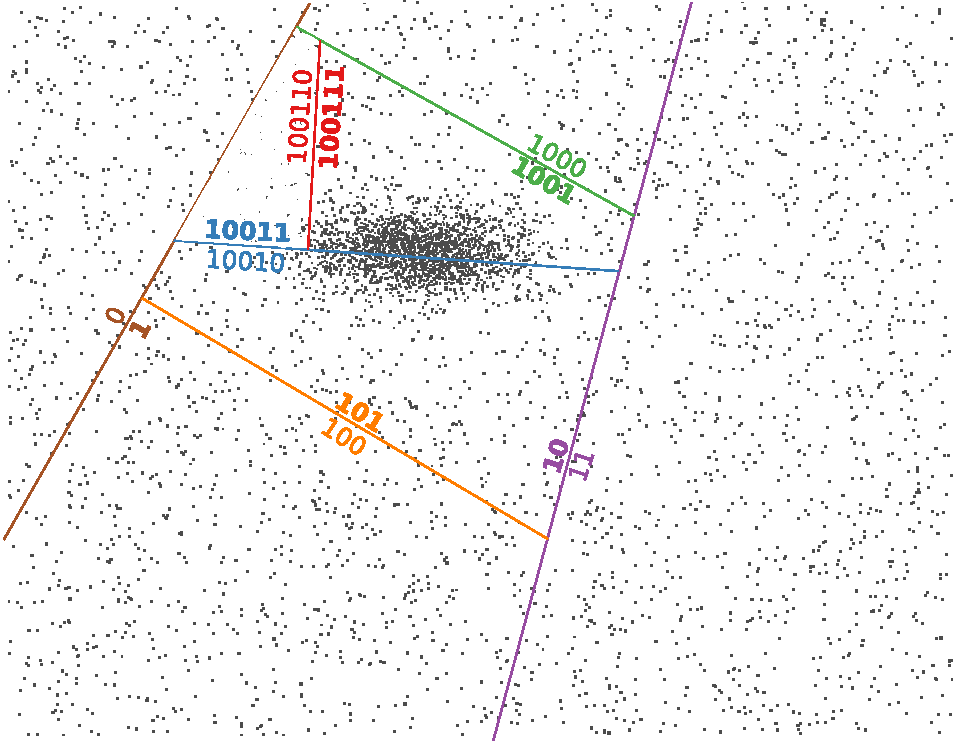
\includegraphics[width=.9\textwidth]{figs/compactcutting}}
\end{figure}
\end{frame}

\begin{frame}[plain]{Adaptive LSH Algorithm}
\begin{Definition}[Sign based Projected LSH]
\label{signbased}
$$
H(X) = \sum sign(P(X))2^n
$$
\end{Definition}

$i=1$\\
$ct,ct\_prev=C\big(\mathbb{H}^{i+1}(x)\big) ,C\big(\mathbb{H}^{i}(x)\big)$\\
\While {$i<n$ \textbf{and} $2ct>ct\_prev$}{
  $ct\_prev,i=ct,i+1$\\
  $ct=C\big(\mathbb{H}^{i}(x)\big)$\\
 }
 \Return $\mathbb{H}^{i}(x)$

\end{frame}

\begin{frame}[plain]{Adaptive LSH Performance}
 \begin{figure}
 \centerline{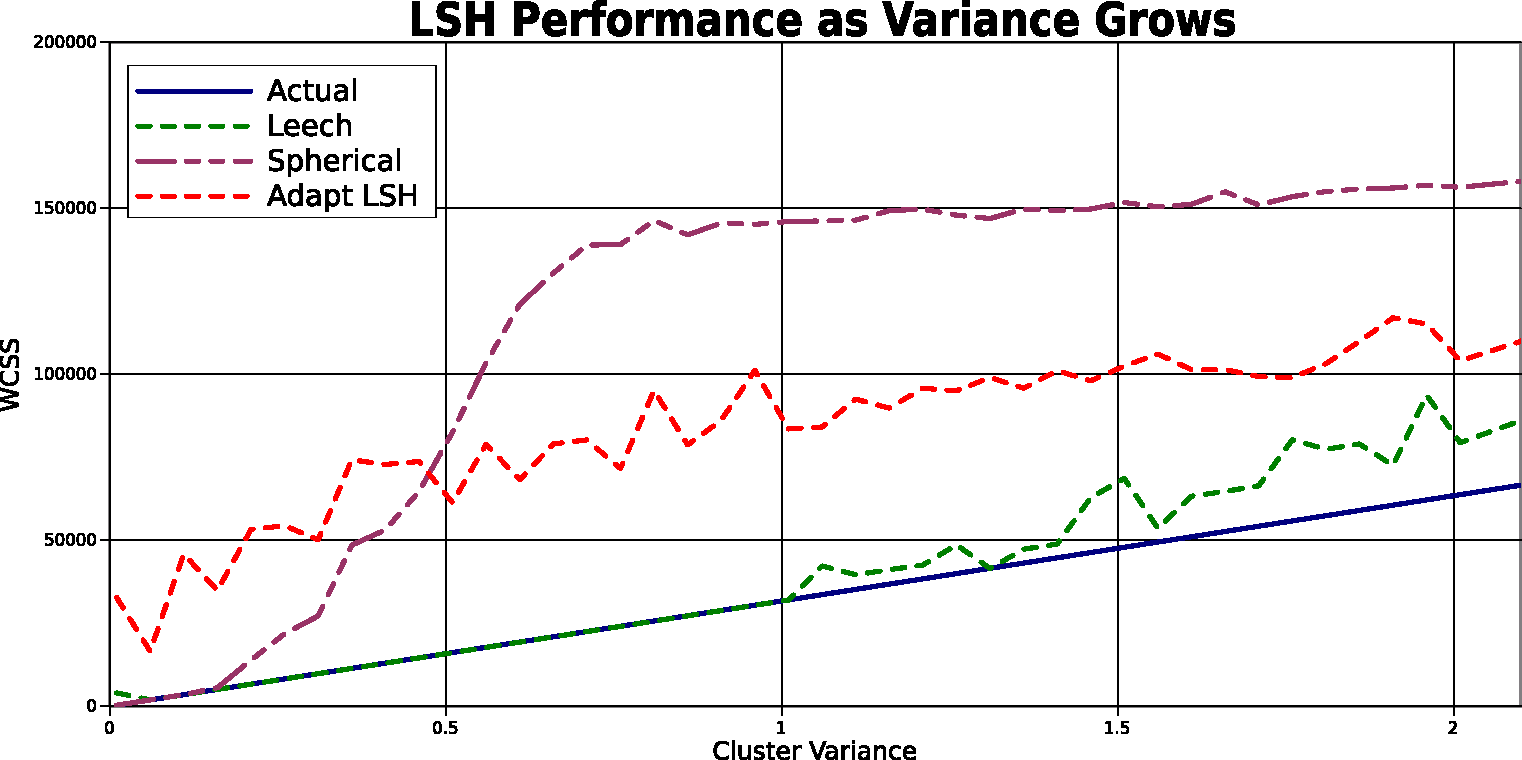
\includegraphics[width=.8\textwidth]{figs/clustervarianceVsDecoders}}
\end{figure}
Worse Than Leech and Spherical
\end{frame}

\begin{frame}[plain]{Evaluate the Neighbors}
\begin{itemize}
  \item Composable hashes let us investigate neighbors
  \item Use neighbor and parent relationships to decide when cuts are useful
  \item Generates a Tree
  \item Tree Based Clustering
\end{itemize}
\end{frame}


\begin{frame}[plain]{Tree Walk RPHash}
\begin{figure}
 \centerline{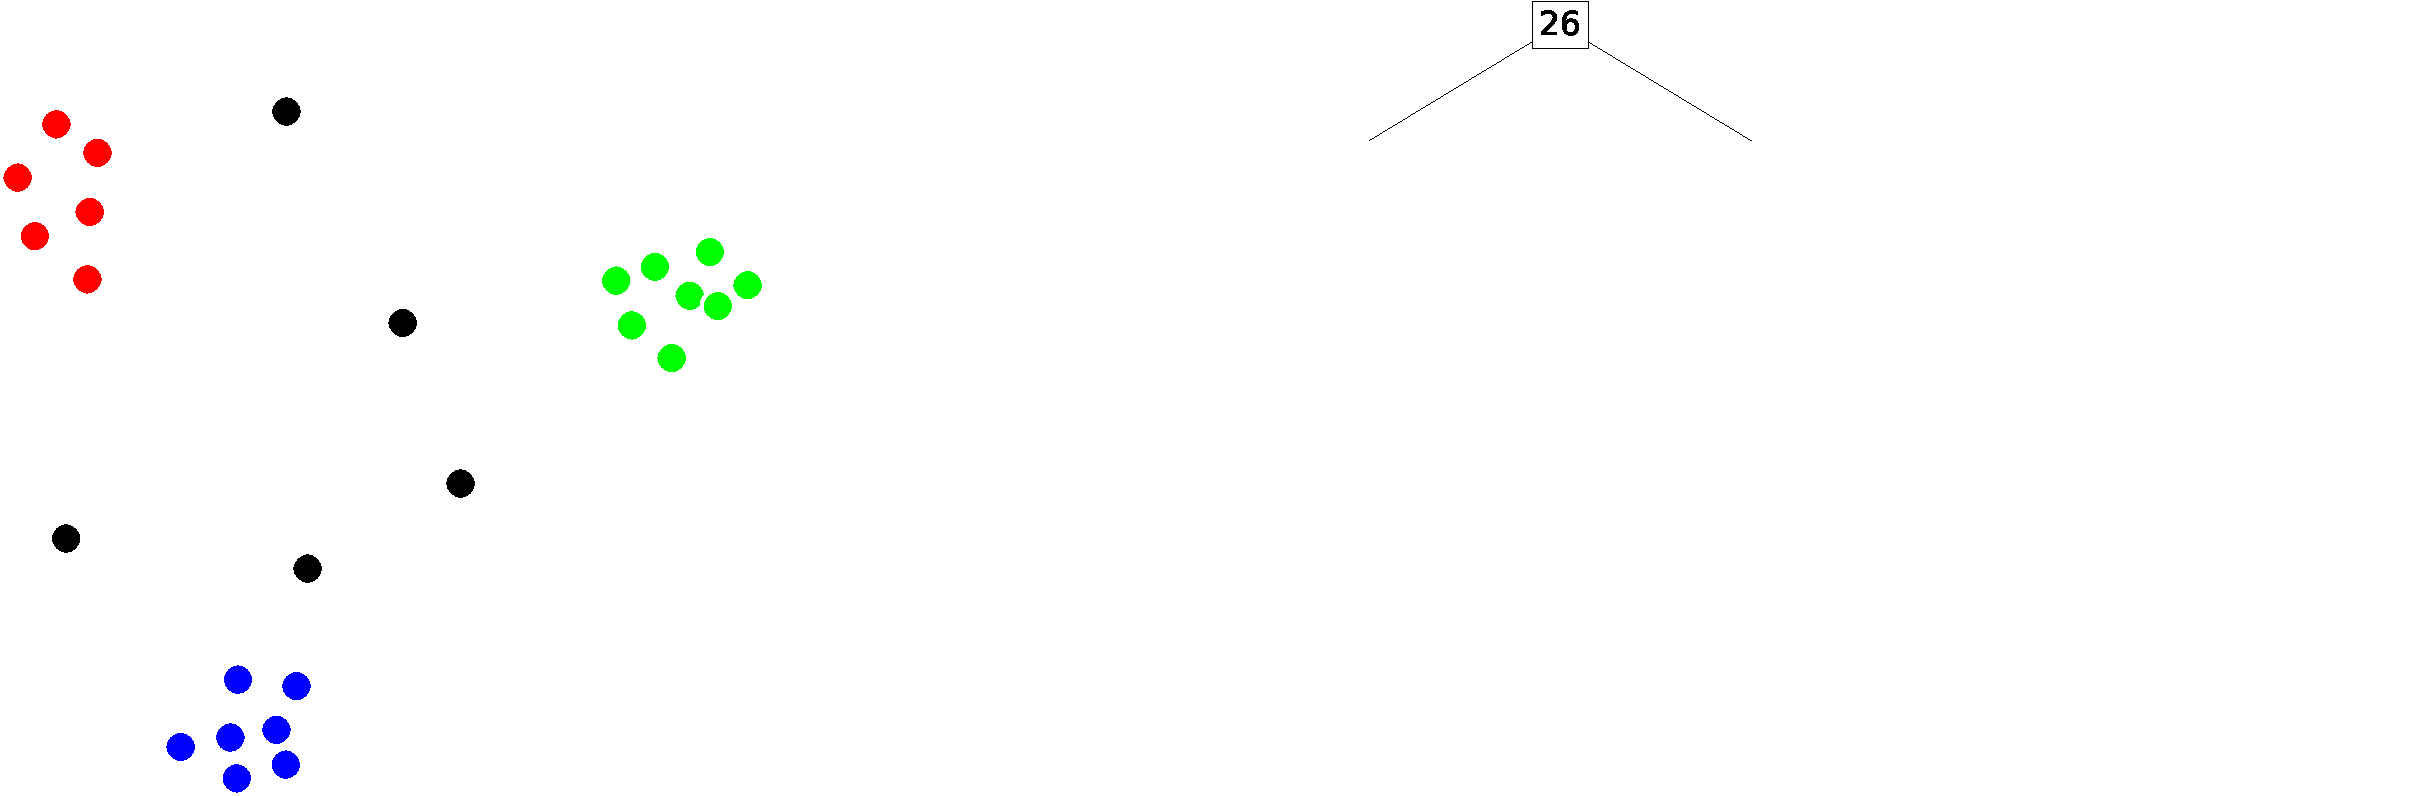
\includegraphics[width=.8\textwidth]{figs/cuts/split1}}
\end{figure}
\end{frame}

\begin{frame}[plain]{Tree Walk RPHash}
\begin{figure}
 \centerline{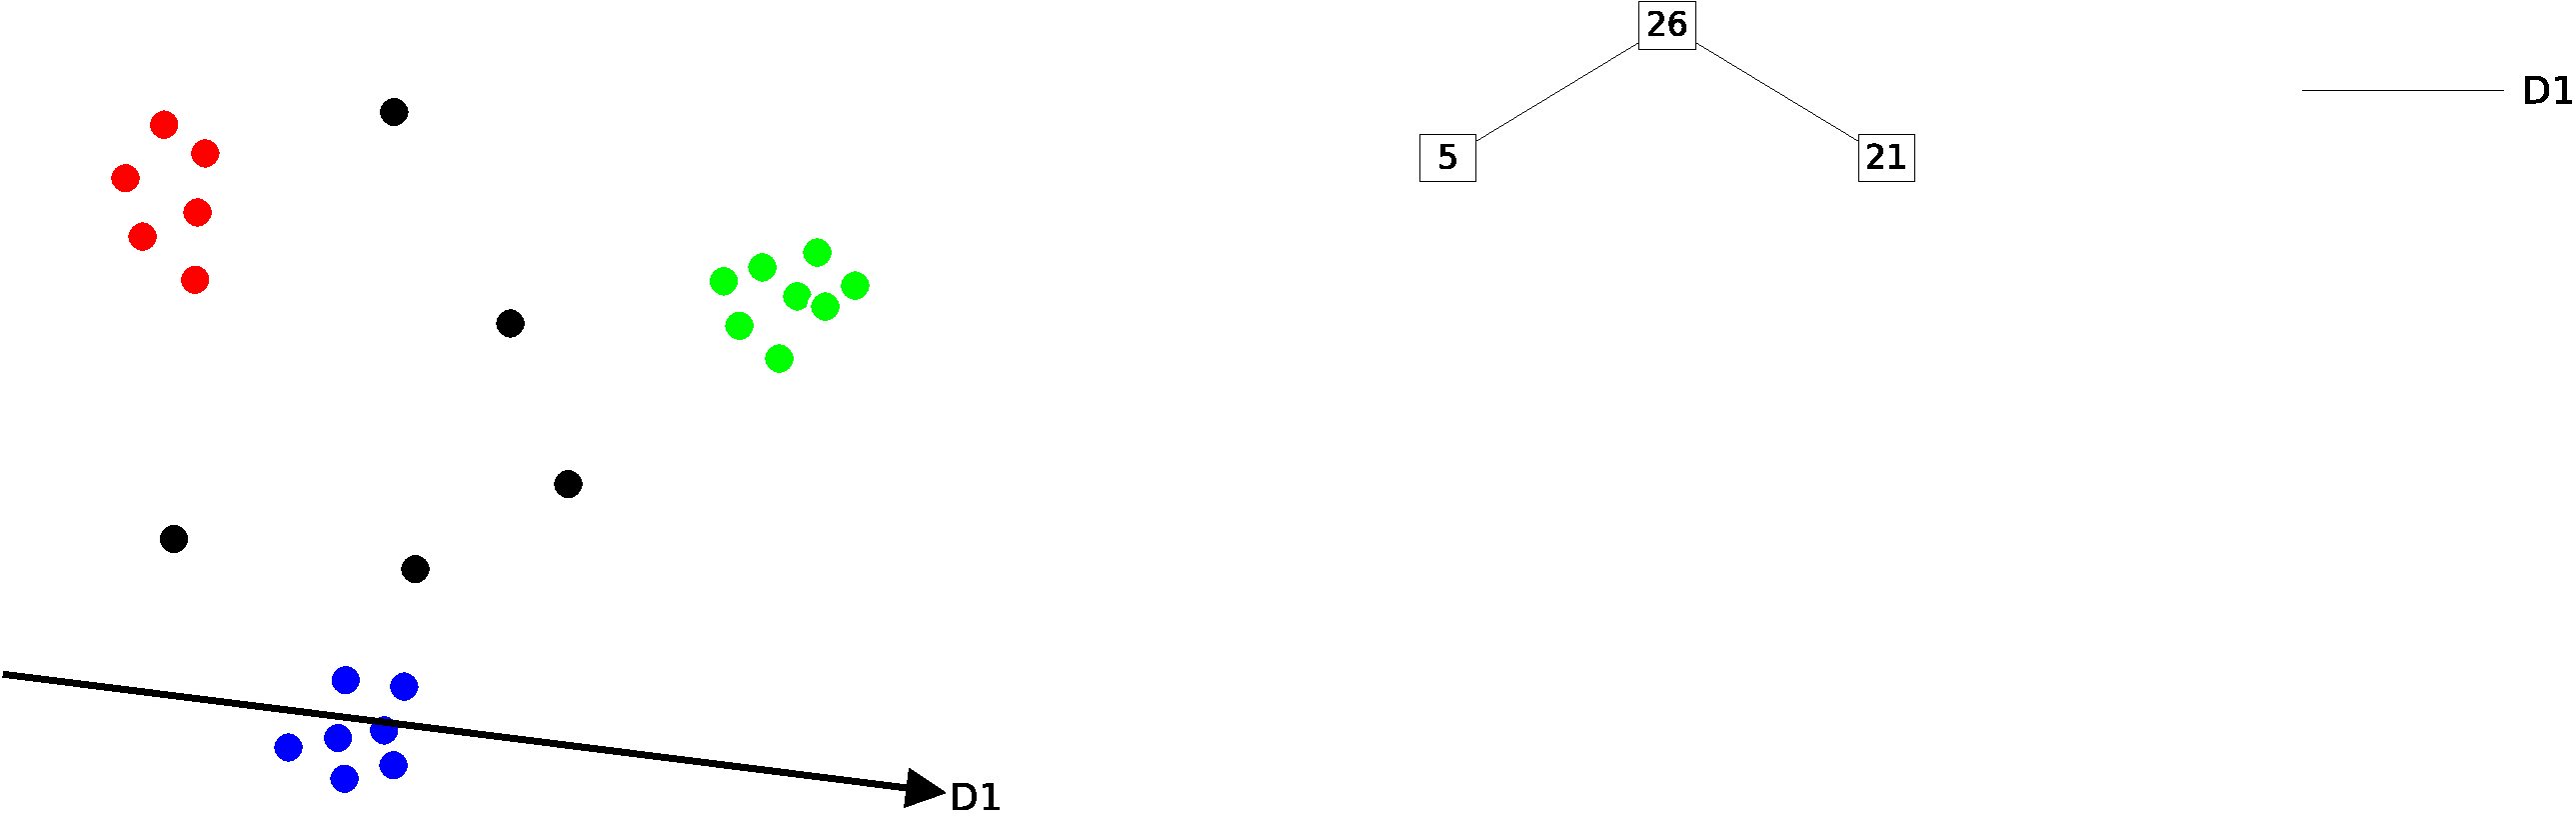
\includegraphics[width=.8\textwidth]{figs/cuts/split2}}
\end{figure}
\end{frame}

\begin{frame}[plain]{Tree Walk RPHash}
\begin{figure}
 \centerline{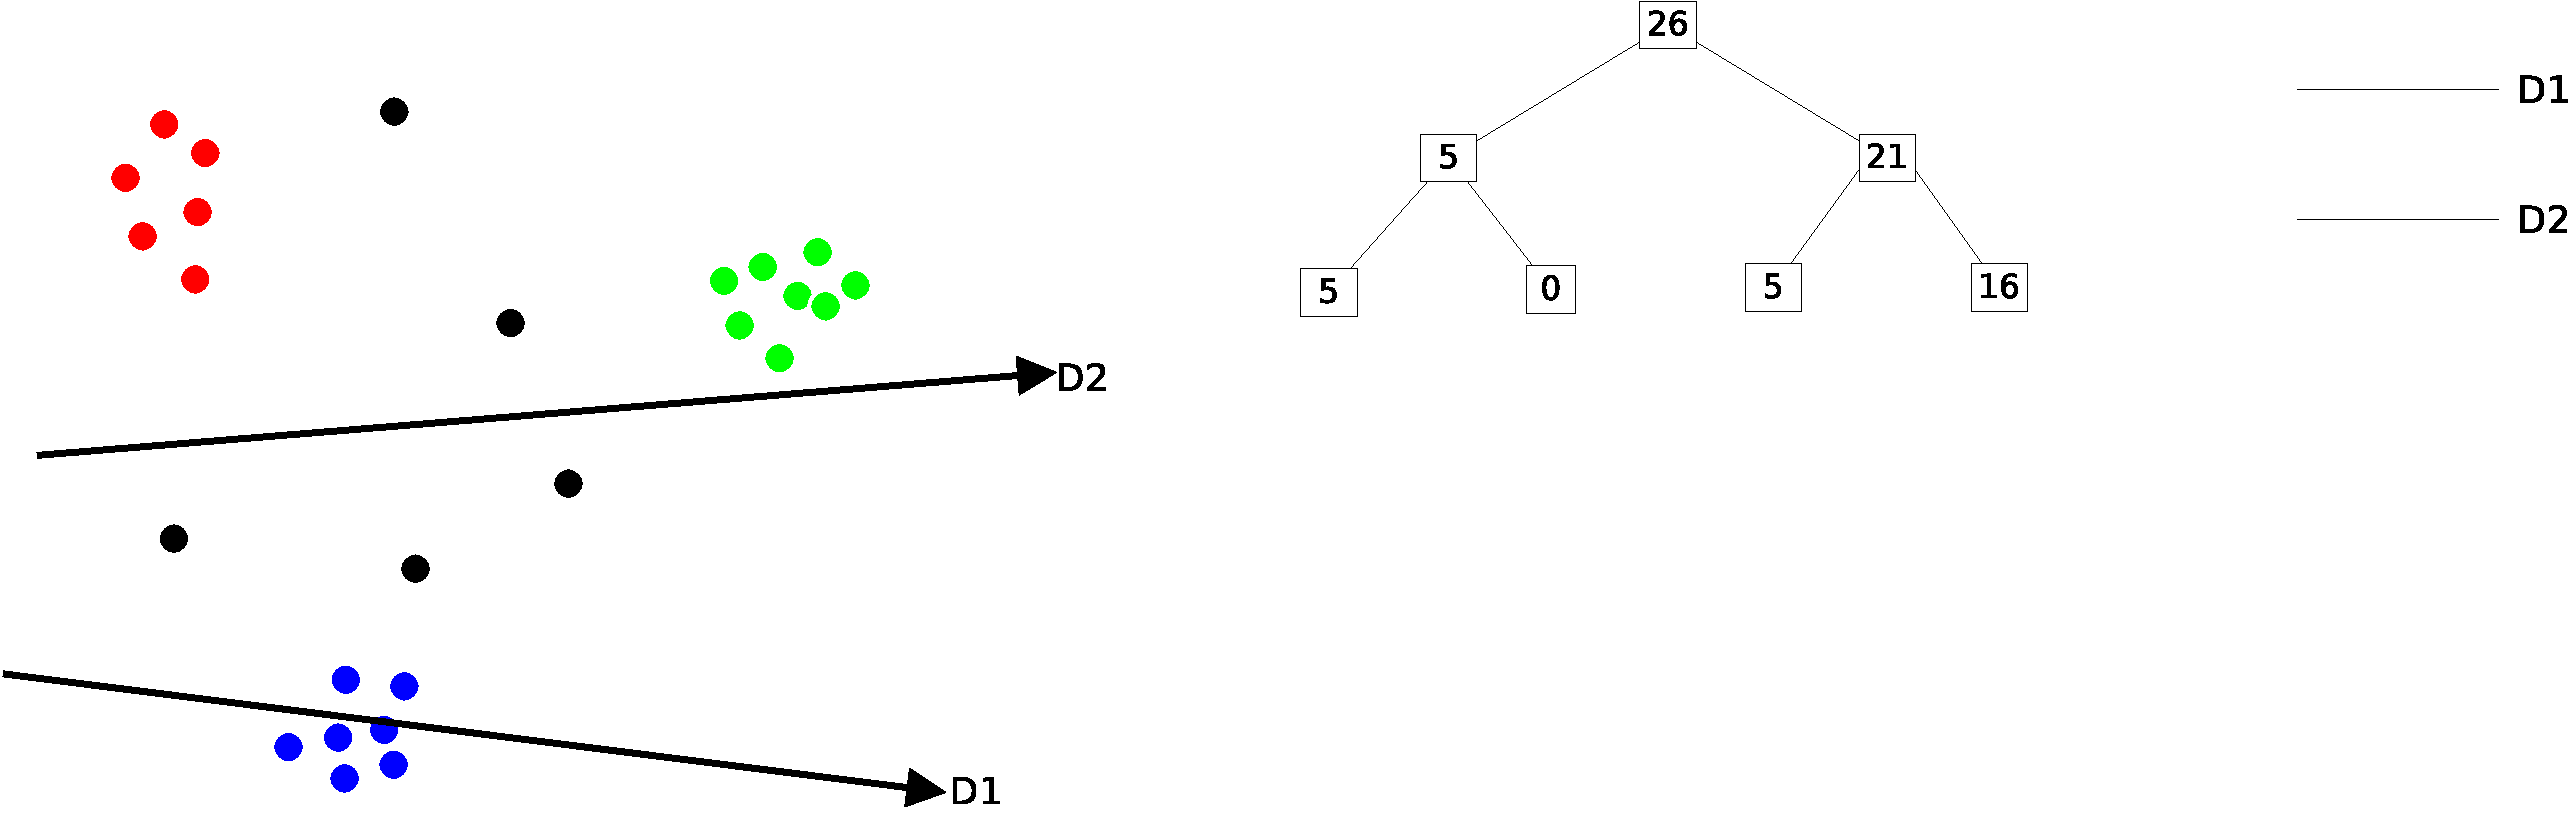
\includegraphics[width=.8\textwidth]{figs/cuts/split3}}
\end{figure}
\end{frame}

\begin{frame}[plain]{Tree Walk RPHash}
\begin{figure}
 \centerline{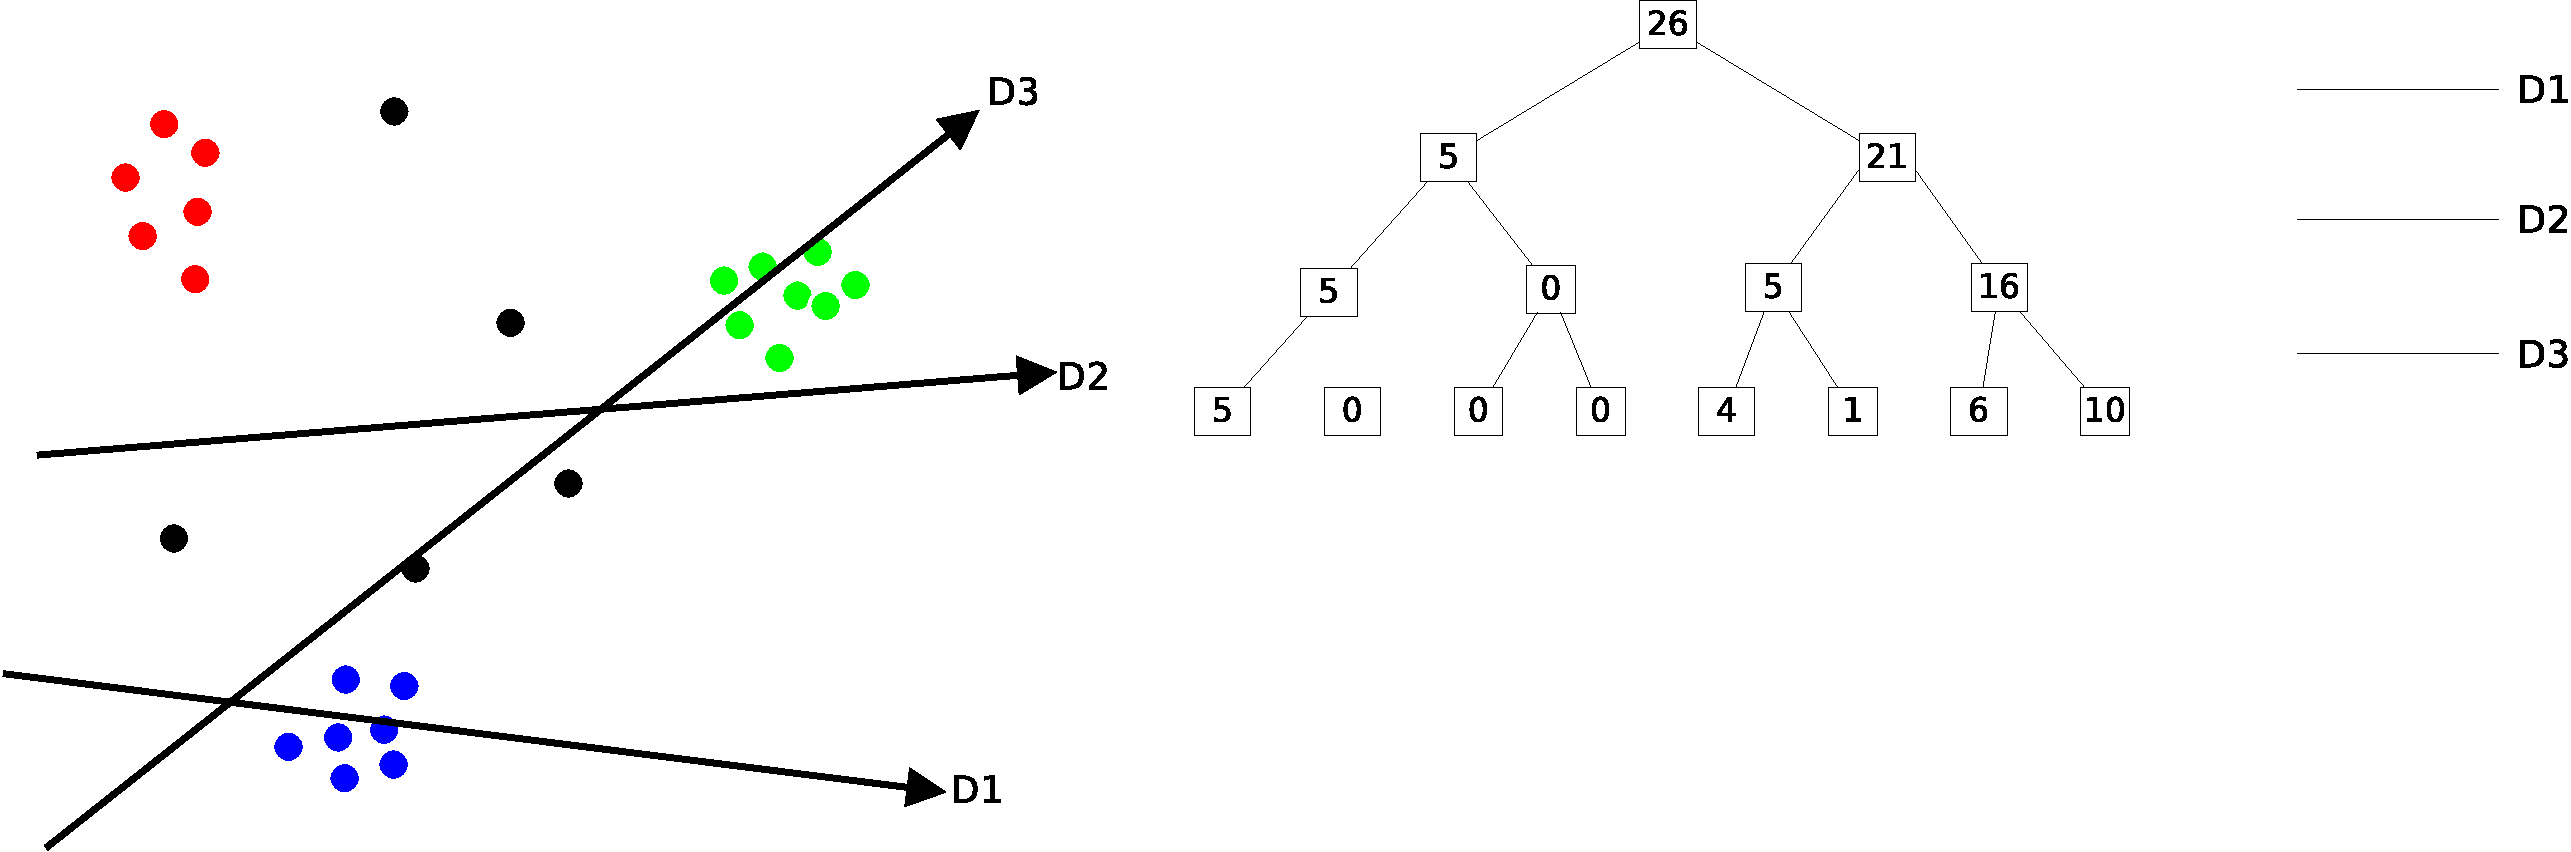
\includegraphics[width=.8\textwidth]{figs/cuts/split4}}
\end{figure}
\end{frame}

\begin{frame}[plain]{Tree Walk RPHash}
\begin{figure}
 \centerline{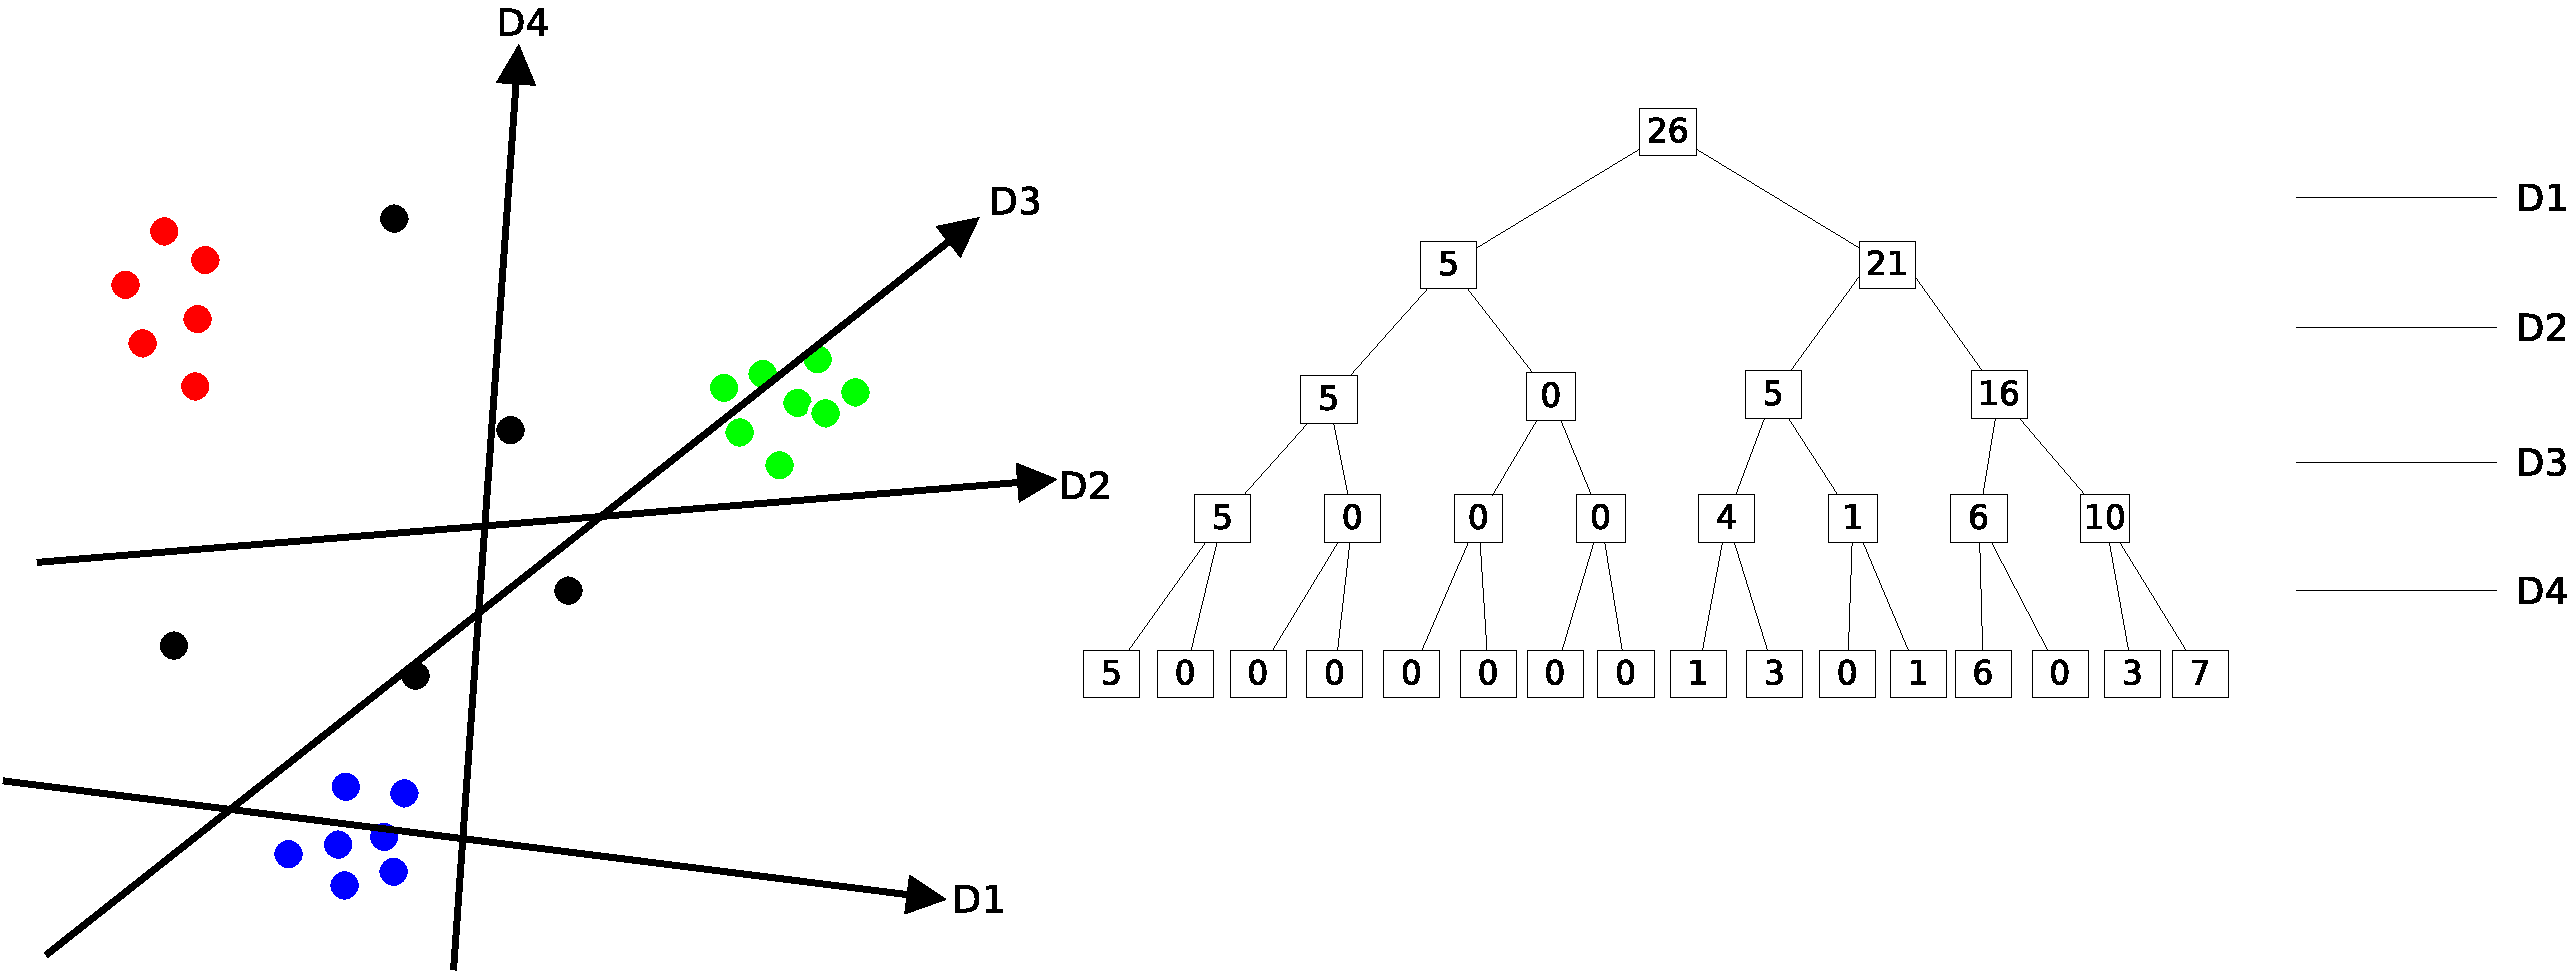
\includegraphics[width=.8\textwidth]{figs/cuts/split5}}
\end{figure}
\end{frame}

\begin{frame}[plain]{Too Big}
\begin{itemize}
 \item The tree is exponential in depth
 \item $\theta(2^d*m)$ - storage complexity
 \item Just need to search, most nodes have low support
 \item Count-Min sketch
\end{itemize}


\end{frame}

\begin{frame}[plain]{Count-Min Tree}
\begin{figure}
 \centerline{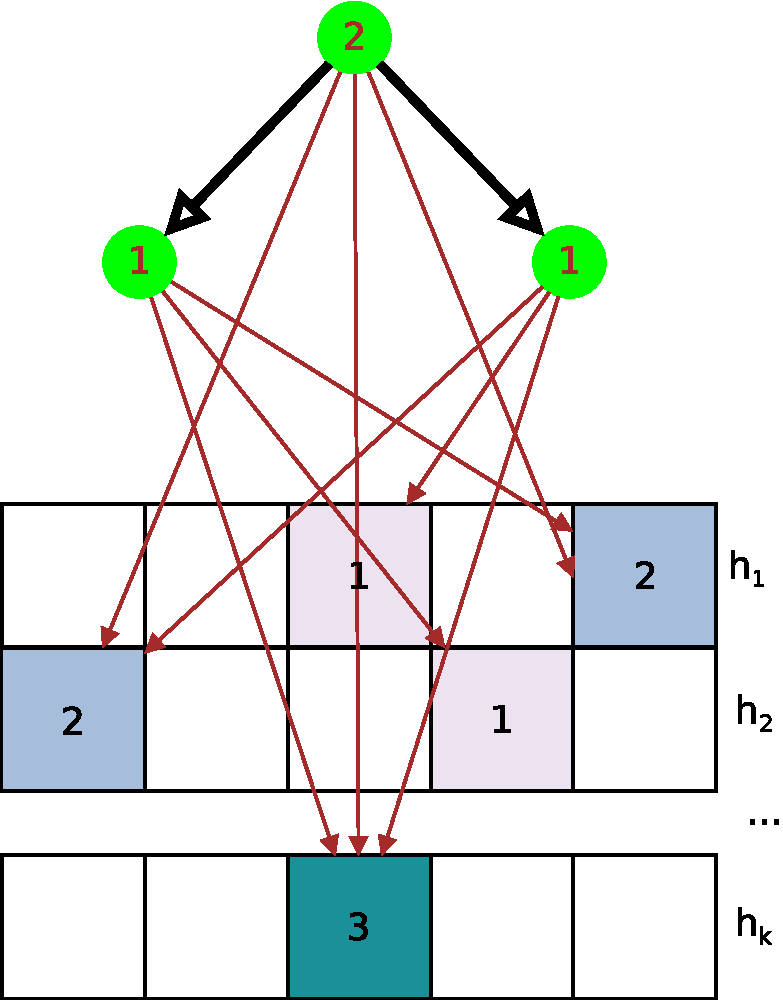
\includegraphics[width=.5\textwidth]{figs/countmintree}}
\end{figure}
\end{frame}

\begin{frame}[plain]{Generate Tree}
  \begin{columns}
    \begin{column}{0.5\textwidth} 
	\ForAll {$x \in X$}{
	$\tilde{x}= \sqrt{\frac{m}{d}}p^{\intercal}x$ 
	$h := \mathbb{H}(\tilde{x})$ 
	\While{$h>0$}{
	  $h = h \gg 1$\\
	  $x' = C[h]+x$\\
	  $C$.add$(h,x')$
	}
	}
    \end{column}
     \begin{column}{0.5\textwidth} 
      $k$ -number of clusters\\
      $X=\{x_1,...,x_n\}$, $x_i \in \mathbb{R}^m$ \\
      $C$- cm-sketch, counts$\rightarrow$vector\\
      $\gg$ - bit shift\\
      $\mathbb{H}(\cdot)$ - LSH Function\\
      $\mathbb{P} = \{p_1,...p_n\}$ - Projectors\\
      $+$-weighted addition
    \end{column}
  \end{columns}
\end{frame}

\begin{frame}[plain]{CLTree for High Dimensional}
\begin{itemize}
 \item TWRP was developed independently, but similar
 \item Concern of CLTree is intersecting clusters
 \item We ignore this concern for high dimensional data and proof the following theorem
\end{itemize}
\begin{Theorem}[Hyper-rectangle Splitting]\label{PrOfCut}
.\\
\begin{minipage}{\textwidth}
The probability of splitting a hyper-rectangular region into two equal mass clusters where subsequent dimensional cuts
are always of the smaller region is 0 as the dimensionality grows to infinity.
$$
\underset{d\rightarrow \infty}{\lim} {{Vol(R) - Vol_{removed}(R)}\over{Vol(R)}} = 0 \text{, }R\text{ is a hyper-rectangle in } \mathbb{R}^d
$$
\end{minipage}
\end{Theorem}
\end{frame}


\begin{frame}[plain]{Evaluate Tree}
\DontPrintSemicolon
\ForAll{$H \in \text{sort}(C\text{.ids})$}
{
\If{$2 C [ H ]< C[ H \gg 1] $}{
  $C[H\gg 1]=0$\\
}
}
$L=[]$\\
\ForAll{$h \in \text{sort} (C \text{.counts})$}
{
	  $L \leftarrow \text{medoid}(C[H])$
}
\Return $L$
\end{frame}


\begin{frame}[plain]{Further Experiments}
 \begin{itemize}
  \item Compare Scalability of algorithms
  \item Parallel Speedup Comparison
  \item Security Evaluation on Real Data
 \end{itemize}
\end{frame} 

\begin{frame}[plain]{Word2Vec TWRP}
\begin{columns}
 \begin{column}{0.65\textwidth} 
 \begin{figure}
 \centerline{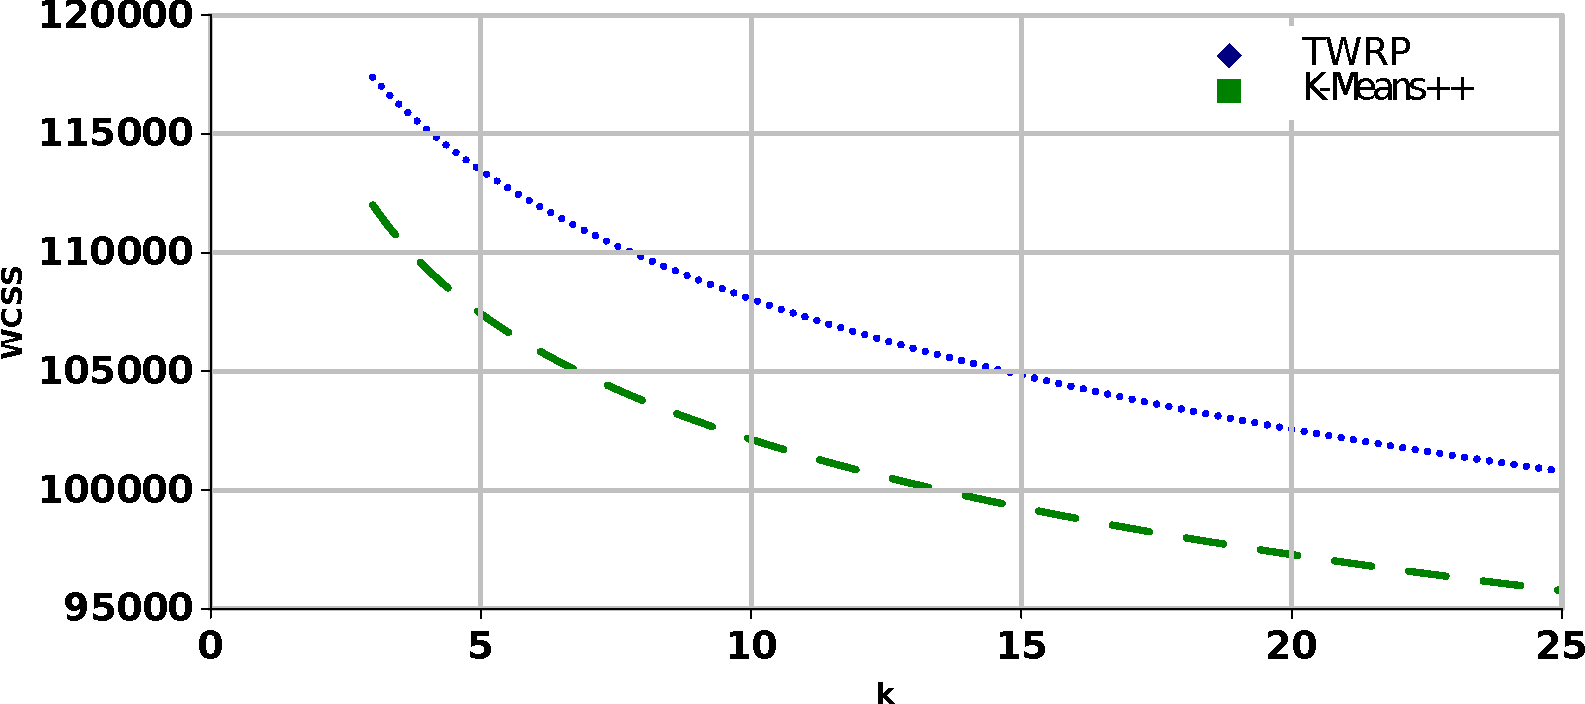
\includegraphics[width=1\textwidth]{figs/w2vwcss}}
\end{figure}
\end{column}
 \begin{column}{0.35\textwidth} 
 \begin{figure}
 \centerline{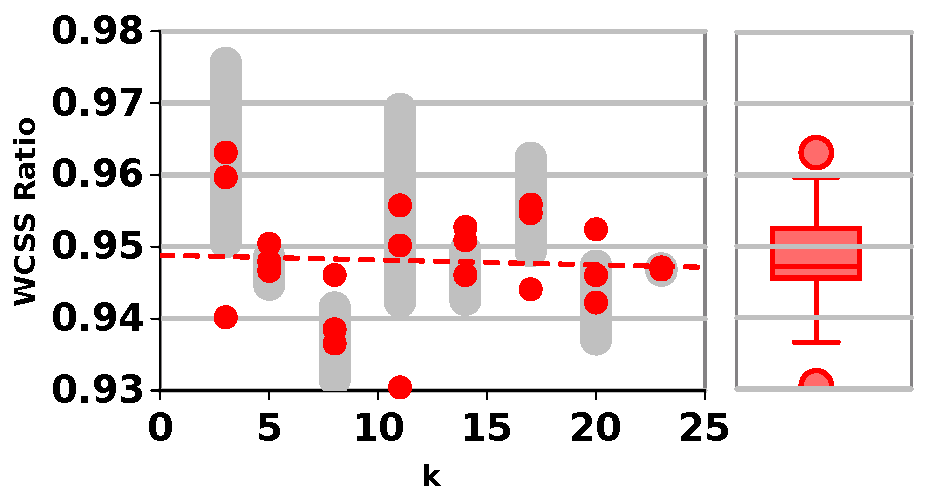
\includegraphics[width=1.3\textwidth]{figs/w2vratio_wcss}}
\end{figure}
\end{column}
\end{columns}
\end{frame}

\begin{frame}[plain]{TWRP Noise}
 \begin{figure}
 \centerline{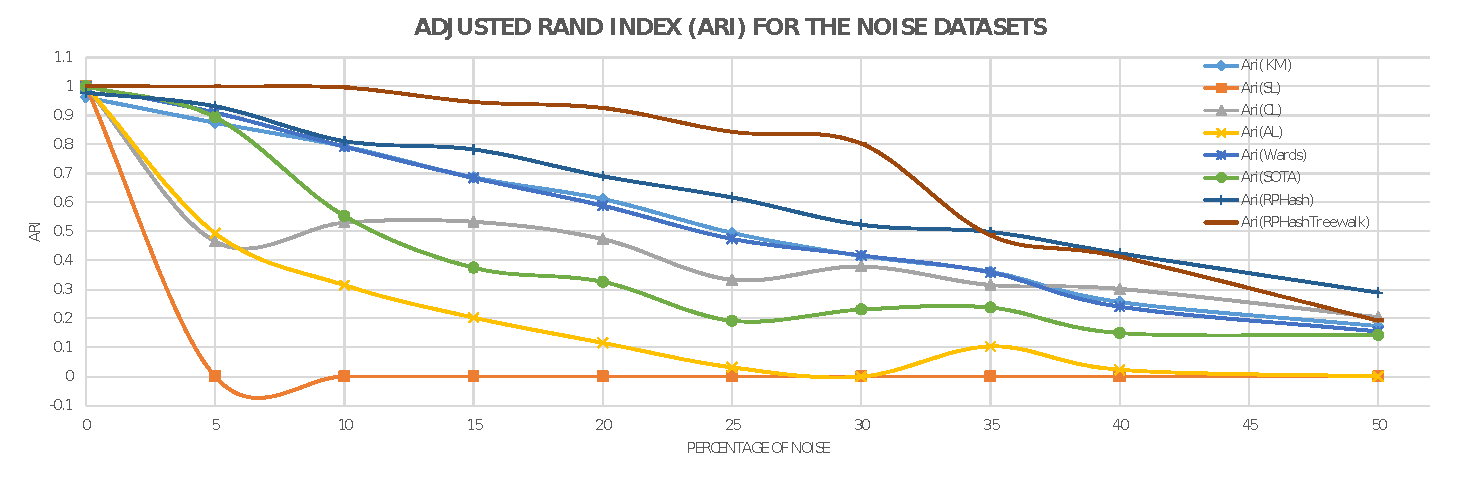
\includegraphics[width=1.1\textwidth]{figs/ari_noise}}
\end{figure}
\end{frame}


\begin{frame}[plain]{Scalability}
 \begin{figure}
 \centerline{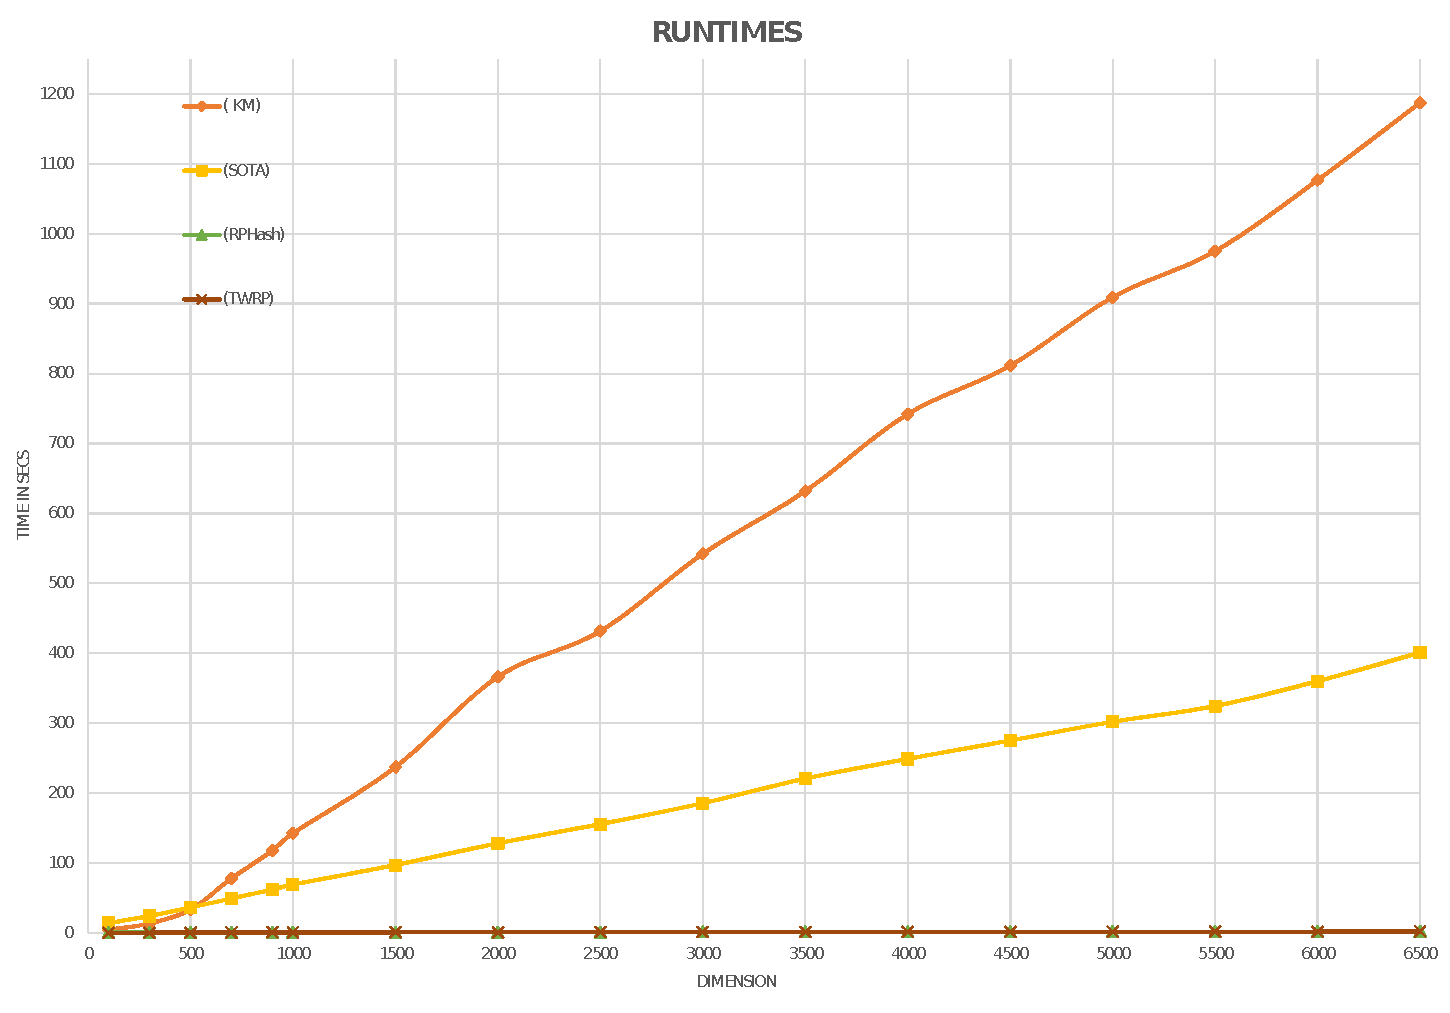
\includegraphics[width=.65\textwidth]{figs/Scalability_Synthetic}}
\end{figure}
\vspace*{-3\bigskipamount}
 \begin{figure}
 \centerline{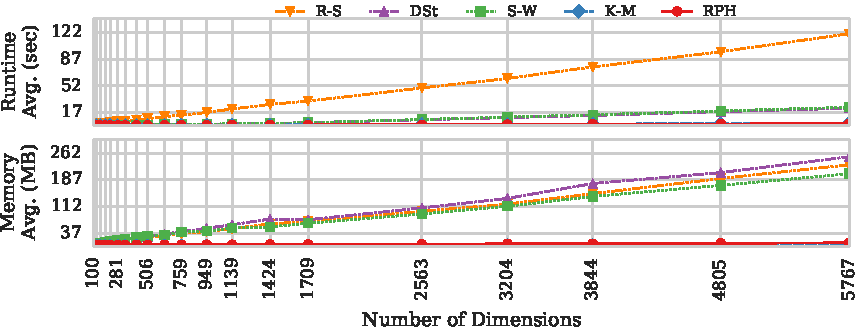
\includegraphics[width=.65\textwidth]{figs/runtimeGraphs}}
\end{figure}
\end{frame}

\begin{frame}[plain]{Theoretical Complexity}
 
 \begin{table}
\centering
\resizebox{\columnwidth}{!}{
\begin{tabular}{|c|c|c|}
\hline
\rowcolor[HTML]{D1FF99} 
\textbf{\emph{LSH} Algorithm} & \textbf{Time Complexity} & \textbf{Space Complexity} \\ \hline
  RPHash & $\Theta(nm)$ & $\Theta(nm)$ \\ \hline
  Streaming RPHash &$\Theta(nm)$ &$\Theta(m\log\log(n)) $ \\ \hline
  TWRP & $\Theta(n m \log^2(n/\varepsilon))$ &  $\Theta(m{e \over \varepsilon}ln({{nlog(d)}\over{(\sqrt{\delta)}}}))$ \\ \hline
 \end{tabular}}
 \end{table}
\end{frame}


\begin{frame}[plain]{Parallelism}
 \begin{figure}
 \centerline{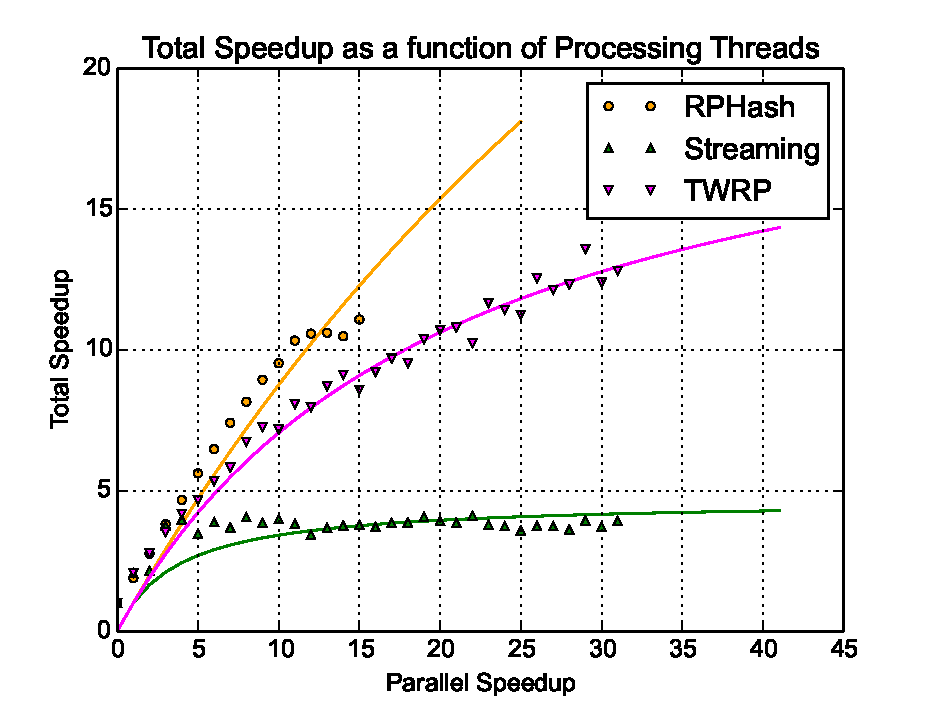
\includegraphics[width=.92\textwidth]{figs/speedup}}
\end{figure}
\end{frame}

\begin{frame}[plain]{Security Assessment}
 \begin{itemize}
 \item \emph{RPHash} increases granularity by projection
 \item Similar to the $l$-diversity metric
 \item Evaluate random projection against data recoverability
  $$ u = \sqrt{{\frac{n}{k}}}R_{d\rightarrow s}^Tv , v' = \sqrt{{\frac{k}{n}}}u^T R_{s\rightarrow d}^{-1} $$
 \item $R$ is non-invertible, best we can do is the Moore-Penrose pseudo-inverse.
\end{itemize}
\end{frame}

\begin{frame}[plain]{Security Assessment (conti.)}
 \begin{figure}
 \centerline{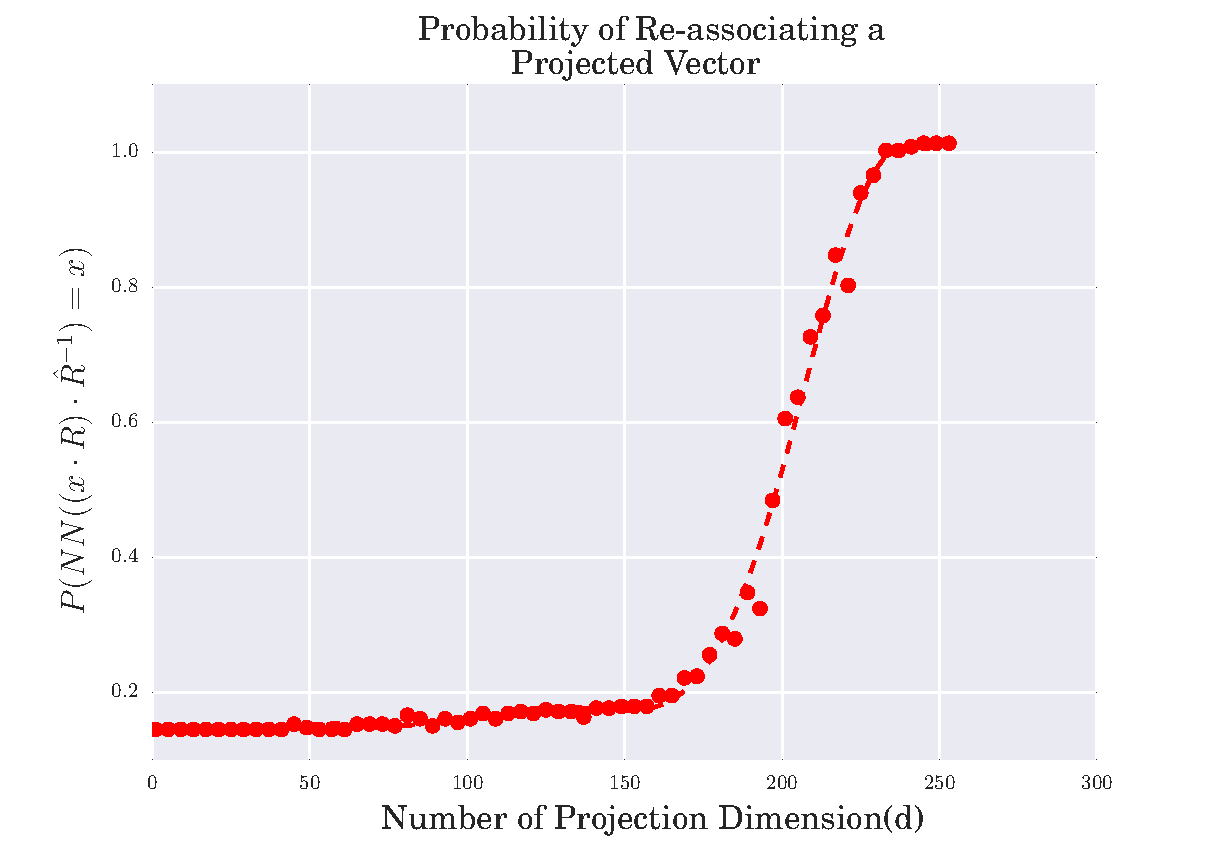
\includegraphics[width=1\textwidth]{figs/recovery}}
\end{figure}
\end{frame}

\begin{frame}[plain]{Conclusions}
\begin{itemize}
 \item Empirically we show that TWRP algorithm and both streaming and standard RPHash are comparable to other clustering methods
 \item our hypothesis that approximate clustering vs local minima clustering holds for many real world and synthetic datasets
\item RPHash has linear complexity, and memory bound and in the streaming case sub-linear memory bound both in theoretically and shown in experiments.
 \end{itemize}
\end{frame}

\begin{frame}[plain]{Future Work}
 \begin{itemize}
  \item Count-Min Cut Tree is interesting for approximate data analysis
  \item Topological Data Analysis could potentially use RPHash for micro-cluster identification to accelerate it
  \item Could accelerate hashing with GPUs
 \end{itemize}
\end{frame}

\begin{frame}[plain]
\begin{center}
\Huge Questions??
\end{center}
\end{frame}

\begin{frame}[allowframebreaks]{References}
       \bibliographystyle{abbrv}
	\bibliography{refs}
\end{frame}

\end{document}
